\documentclass{ieeetj}
\usepackage{cite}
\usepackage{amsmath,amssymb,amsfonts,amsthm,mathtools}
\usepackage{graphicx,color}
\usepackage{xcolor}
\usepackage{booktabs}
\usepackage{multirow}
\usepackage{url}
\usepackage{bm}
\usepackage{tikz}
\usepackage{hyperref}
\hypersetup{hidelinks=true}
\AtBeginDocument{\definecolor{tmlcncolor}{cmyk}{0.93,0.59,0.15,0.02}\definecolor{NavyBlue}{RGB}{0,86,125}}

% Space-saving adjustments
\setlength{\textfloatsep}{8pt plus 2pt minus 2pt}
\setlength{\floatsep}{6pt plus 2pt minus 2pt}
\setlength{\abovecaptionskip}{4pt}
\setlength{\belowcaptionskip}{2pt}
\setlength{\abovedisplayskip}{5pt plus 2pt minus 2pt}
\setlength{\belowdisplayskip}{5pt plus 2pt minus 2pt}
\setlength{\intextsep}{6pt plus 2pt minus 2pt}
\usetikzlibrary{arrows.meta,positioning,fit,backgrounds,calc,decorations.pathreplacing}
\def\BibTeX{{\rm B\kern-.05em{\sc i\kern-.025em b}\kern-.08em
    T\kern-.1667em\lower.7ex\hbox{E}\kern-.125emX}}
\def\OJlogo{}
\def\seclogo{}
\def\authorrefmark#1{\ensuremath{^{\textbf{#1}}}}
\newtheorem{theorem}{Theorem}
\newtheorem{corollary}{Corollary}

\begin{document}
\receiveddate{}
\reviseddate{}
\accepteddate{}
\publisheddate{}
\currentdate{}
\doiinfo{}
\markboth{}{Anonymous Submission}
\title{Clinically Constrained Cooperative Neuro-Symbolic Post-Correction for OCT Denoising}
\author{Anonymous Author(s)}
\affil{Anonymous Affiliation}
\corresp{Correspondence withheld for double-blind review.}
\authornote{This manuscript is prepared for double-blind review.}

\begin{abstract}
Optical coherence tomography (OCT) denoisers are typically optimized for pixel fidelity, yet the resulting images can still lose contrast, boundary definition, and layer visibility that matter clinically. This paper does not introduce a new denoising backbone. Instead, it studies a clinically constrained post-correction layer that can be attached to a pretrained denoiser and can improve clinically relevant image attributes without discarding the backbone's pixel-level strength. We present \textbf{CoopNS-OCT}, a cooperative neuro-symbolic wrapper composed of a lightweight backbone-specific confidence head, multiplicative and additive correctors, and a differentiable fuzzy negotiator driven by six explicitly defined ground-truth-free predicates. For each predicate we specify both a scalar score and a spatial failure map, which addresses reproducibility at the level of the negotiator input. We further prove that the negotiated allocation map is Lipschitz-stable with respect to predicate perturbations and derive a margin-based lower bound showing when tissue-only gated correction improves contrast-to-noise ratio (CNR) despite bounded background leakage. The wrapper adds only 0.168M trainable parameters (about 2.4\% overhead relative to a 7M backbone). On PKU37 and leave-one-out Duke17/Duke2013 evaluation, CoopNS-OCT improves CNR by 10--15\% and boundary sharpness by 2.5--11\% with controlled PSNR trade-offs of 0.25--0.80 dB. The same cooperative logic transfers across NAFNet, DnCNN, SwinIR, and KBNet after only adapting the confidence head, supporting a clearly backbone-\emph{modular} interpretation.
\end{abstract}

\begin{IEEEkeywords}
Optical coherence tomography, image denoising, neuro-symbolic reasoning, fuzzy logic, interpretable image restoration, modular post-correction, clinical quality assessment.
\end{IEEEkeywords}

\maketitle

\section{Introduction}
\label{sec:introduction}
\IEEEPARstart{O}{ptical} coherence tomography (OCT) is the dominant non-invasive imaging modality for retinal diagnostics~\cite{huang1991optical}. OCT images are degraded by multiplicative speckle noise~\cite{goodman2007speckle} that obscures layer boundaries, reduces contrast, and limits the reliability of downstream analyses such as layer segmentation~\cite{devalla2018drunet}.

\subsection{Motivation}
Despite rapid progress in deep denoisers~\cite{zhang2017beyond,chen2022simple,liang2021swinir,krull2019noise2void}, most OCT restoration pipelines still optimize denoising as pixel regression. This is often mismatched to clinical use: a backbone can gain PSNR while degrading tissue-background separability, boundary sharpness, or layer visibility. A second problem is interpretability. When a post-processing module changes an OCT scan, clinicians and reviewers should be able to inspect \emph{why} and \emph{where} the correction was applied, rather than treating the adjustment as a black-box residual.

The central question of this paper is therefore not ``Can we invent yet another OCT backbone?'' but rather: \emph{Can a clinically meaningful correction policy be formalized as explicit spatial predicates, routed through stable symbolic logic, and attached to strong pretrained denoisers with bounded risk to fidelity?} This framing is important because it moves the contribution away from claiming novelty for standard components in isolation. The technical contribution lies in the wrapper: the predicate formalization, the cooperative allocation mechanism, and the safety-gated correction rule.

\subsection{Contributions}
We propose \textbf{CoopNS-OCT}, a cooperative neuro-symbolic OCT post-correction framework. The paper is positioned as a systems-and-methodology contribution on clinically constrained correction, not as a claim that Sobel edges, fuzzy logic, or uncertainty heads are individually novel. Our contributions are:

\begin{enumerate}
\item \textbf{Backbone-modular cooperative correction} (Section~\ref{sec:cooperative}): a frozen denoising backbone is augmented by a lightweight confidence head, a multiplicative gain corrector, and an additive edge recovery module. The correction layer is shared across backbone families; only the confidence head depends on backbone feature dimensionality. We therefore make the narrower and technically defensible claim of \emph{modularity}, not universal architecture agnosticism.

\item \textbf{Explicit predicate-to-map formalization} (Section~\ref{sec:negotiator}): six ground-truth-free clinical predicates are specified as closed-form score functions together with spatial failure maps. This gives reproducible negotiator inputs rather than qualitative descriptors such as ``edge-to-flat ratio'' or ``vertical consistency'' without formulas.

\item \textbf{Stable symbolic allocation with theorem-backed transfer behavior} (Section~\ref{sec:negotiator}): the negotiator uses differentiable Lukasiewicz logic~\cite{vankrieken2022analyzing} to combine predicate failures into a per-pixel allocation rule. We prove the allocation is Lipschitz-stable with respect to perturbations of the predicate vector, which explains why the same negotiated policy remains well behaved when the backbone is replaced and the calibrated predicate scores shift slightly.

\item \textbf{Safety-gated correction with clinically meaningful guarantees} (Sections~\ref{sec:cnr}--\ref{sec:formal}): tissue-aware gating, bounded perturbation, energy descent, and Pareto-style non-degradation are combined with a margin-based CNR result that makes explicit when the wrapper improves clinically relevant contrast despite bounded background leakage. Cross-dataset leave-one-out (LOO) evaluation on Duke17 and Duke2013 shows consistent gains across four strong learned backbones.
\end{enumerate}

Fig.~\ref{fig:architecture} illustrates the overall architecture. A frozen denoiser produces $\hat{\mathbf{x}}_\text{base}$, a confidence head estimates per-pixel uncertainty, and two lightweight correctors propose multiplicative and additive refinements. A symbolic negotiator then decides where the gain pathway should be active, while safety constraints determine how strongly the corrected candidate may deviate from the backbone output.

The remainder of the paper is organized as follows. Section~\ref{sec:related} reviews related work. Section~\ref{sec:cooperative} describes the modular correction wrapper. Section~\ref{sec:negotiator} formalizes the predicate maps and symbolic allocation. Section~\ref{sec:cnr} presents the safety-gated correction rule and guarantees. Section~\ref{sec:experiments} reports the evaluation, and Section~\ref{sec:conclusion} concludes.

\begin{figure*}[t]
\centering
\resizebox{\textwidth}{!}{%
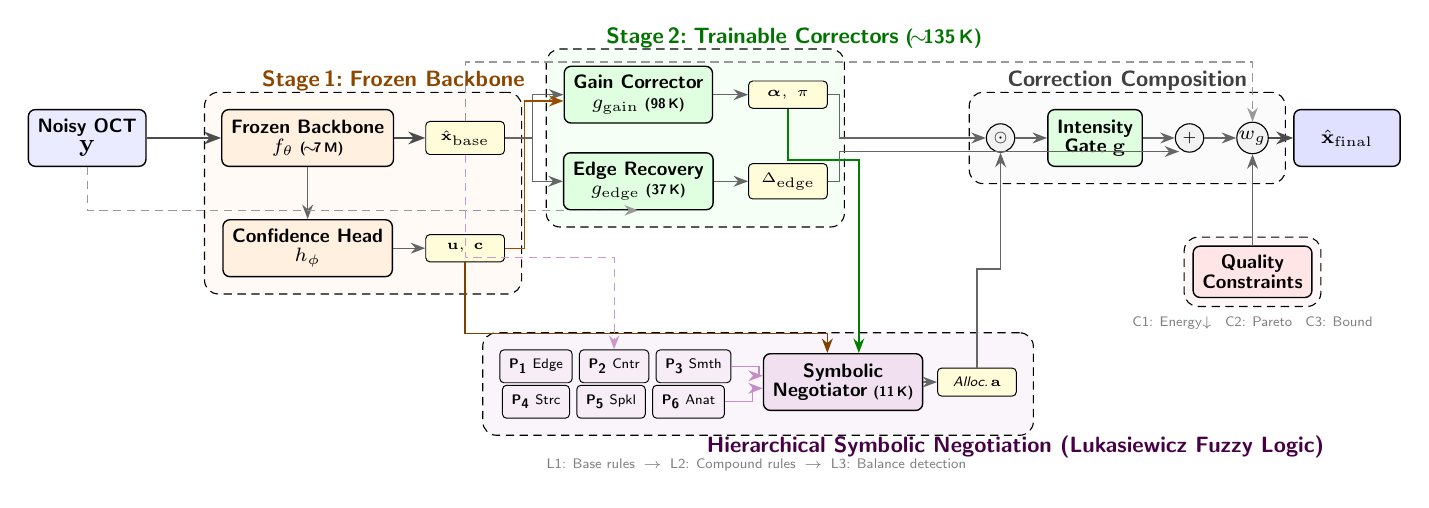
\begin{tikzpicture}[
    >=Stealth,
    inout/.style={draw, rounded corners=2.5pt, fill=blue!8, minimum height=0.72cm, minimum width=1.35cm, font=\sffamily\scriptsize\bfseries, align=center, line width=0.5pt},
    frozenblk/.style={draw, rounded corners=2.5pt, fill=orange!12, minimum height=0.72cm, minimum width=1.7cm, font=\sffamily\scriptsize\bfseries, align=center, line width=0.5pt},
    corrblk/.style={draw, rounded corners=2.5pt, fill=green!12, minimum height=0.72cm, minimum width=1.55cm, font=\sffamily\scriptsize\bfseries, align=center, line width=0.5pt},
    symbblk/.style={draw, rounded corners=2.5pt, fill=violet!12, minimum height=0.72cm, minimum width=1.55cm, font=\sffamily\scriptsize\bfseries, align=center, line width=0.5pt},
    predblk/.style={draw, rounded corners=1.5pt, fill=violet!7, minimum height=0.3cm, minimum width=0.8cm, font=\sffamily\tiny, align=center, line width=0.35pt},
    constblk/.style={draw, rounded corners=2.5pt, fill=red!10, minimum height=0.65cm, minimum width=1.35cm, font=\sffamily\scriptsize\bfseries, align=center, line width=0.5pt},
    mapblk/.style={draw, rounded corners=1.5pt, fill=yellow!15, minimum height=0.34cm, minimum width=1.0cm, font=\sffamily\tiny\itshape, align=center, line width=0.35pt},
    opcirc/.style={draw, circle, fill=gray!10, minimum size=0.36cm, font=\sffamily\tiny\bfseries, inner sep=0pt, line width=0.4pt},
    arr/.style={->, line width=0.5pt, color=black!60},
    arrbold/.style={->, line width=0.7pt, color=black!70},
    arrdash/.style={->, line width=0.45pt, color=black!40, densely dashed},
    lbl/.style={font=\sffamily\tiny\color{black!50}, align=center},
    glbl/.style={font=\sffamily\tiny\bfseries},
    gbox/.style={draw, densely dashed, rounded corners=5pt, line width=0.4pt, inner sep=6pt},
]
% Input
\node[inout] (input) at (0, 0) {Noisy OCT\\[-1pt]{\small$\mathbf{y}$}};
% Frozen Backbone
\node[frozenblk] (bbone) at (2.8, 0) {Frozen Backbone\\[-1pt]$f_\theta$\;{\tiny($\!\sim\!$7\,M)}};
\node[frozenblk] (conf) at (2.8, -1.4) {Confidence Head\\[-1pt]$h_\phi$};
\node[mapblk] (xbase) at (4.8, 0) {$\hat{\mathbf{x}}_{\mathrm{base}}$};
\node[mapblk] (uc) at (4.8, -1.4) {$\mathbf{u},\;\mathbf{c}$};
\draw[arrbold] (input) -- (bbone);
\draw[arrbold] (bbone) -- (xbase);
\draw[arr] (bbone) -- (conf);
\draw[arr] (conf) -- (uc);
% Correctors
\node[corrblk] (gain) at (7.0, 0.55) {Gain Corrector\\[-1pt]$g_{\mathrm{gain}}$\;{\tiny(98\,K)}};
\node[corrblk] (edge) at (7.0, -0.55) {Edge Recovery\\[-1pt]$g_{\mathrm{edge}}$\;{\tiny(37\,K)}};
\node[mapblk] (gainout) at (8.9, 0.55) {$\boldsymbol{\alpha},\;\pi$};
\node[mapblk] (edgeout) at (8.9, -0.55) {$\Delta_{\mathrm{edge}}$};
\draw[arr] (xbase.east) -- ++(0.35cm,0) coordinate (xfan) |- (gain.west);
\draw[arr] (xfan) |- (edge.west);
\draw[arrdash] (input.south) -- ++(0,-0.55cm) -| ([xshift=-0.2cm]edge.south) -- (edge.south);
\draw[arr, color=orange!60!black] (uc.east) -- ++(0.25cm,0) |- ([yshift=-0.08cm]gain.west);
\draw[arr] (gain) -- (gainout);
\draw[arr] (edge) -- (edgeout);
% Predicates
\node[predblk] (p1) at (5.7, -2.9) {\textbf{P\textsubscript{1}} Edge};
\node[predblk, right=0.08cm of p1] (p2) {\textbf{P\textsubscript{2}} Cntr};
\node[predblk, right=0.08cm of p2] (p3) {\textbf{P\textsubscript{3}} Smth};
\node[predblk] (p4) at (5.7, -3.35) {\textbf{P\textsubscript{4}} Strc};
\node[predblk, right=0.08cm of p4] (p5) {\textbf{P\textsubscript{5}} Spkl};
\node[predblk, right=0.08cm of p5] (p6) {\textbf{P\textsubscript{6}} Anat};
\draw[arrdash, color=violet!40] (xbase.south) -- ++(0,-1.3cm) -| (p2.north);
% Symbolic Negotiator
\node[symbblk] (negot) at (9.6, -3.1) {Symbolic\\[-1pt]Negotiator\;{\tiny(11\,K)}};
\draw[arr, color=violet!45] (p3.east) -- ++(0.35cm,0) |- ([yshift=0.08cm]negot.west);
\draw[arr, color=violet!45] (p6.east) -- ++(0.35cm,0) |- ([yshift=-0.08cm]negot.west);
\draw[arr, color=green!50!black] (gainout.south) -- ++(0,-0.65cm) -| ([xshift=0.2cm]negot.north);
\draw[arr, color=orange!50!black] (uc.south) -- ++(0,-0.9cm) -| ([xshift=-0.2cm]negot.north);
\node[mapblk] (alloc) at (11.3, -3.1) {Alloc.\,$\mathbf{a}$};
\draw[arr] (negot) -- (alloc);
\node[lbl] (lvlannot) at (8.5, -4.15) {L1: Base rules\;\;$\rightarrow$\;\;L2: Compound rules\;\;$\rightarrow$\;\;L3: Balance detection};
% Correction Composition
\node[opcirc] (odot) at (11.6, 0) {$\odot$};
\node[corrblk, minimum width=1.2cm] (igate) at (12.8, 0) {Intensity\\[-1pt]Gate\;$\mathbf{g}$};
\node[opcirc] (plus) at (14.0, 0) {$+$};
\node[opcirc, minimum size=0.4cm] (wg) at (14.8, 0) {\scriptsize$w_g$};
\node[inout, fill=blue!12] (final) at (16.0, 0) {$\hat{\mathbf{x}}_{\mathrm{final}}$};
\draw[arr] (gainout.east) -- ++(0.15cm,0) |- (odot.west);
\draw[arr] (alloc.north) -- ++(0,1.25cm) -| (odot.south);
\draw[arr] (odot) -- (igate);
\draw[arr] (igate) -- (plus);
\draw[arr] (plus) -- (wg);
\draw[arrbold] (wg) -- (final);
\draw[arr] (edgeout.east) -- ++(0.15cm,0) |- ([yshift=-0.04cm]plus.south west);
\draw[arrdash] (xbase.north) -- ++(0,0.75cm) -| (wg.north);
% Quality Constraints
\node[constblk] (qconst) at (14.8, -1.7) {Quality\\[-1pt]Constraints};
\draw[arr] (qconst) -- (wg);
\node[lbl, below=0.12cm of qconst] {C1: Energy$\downarrow$\;\; C2: Pareto\;\; C3: Bound};
% Group boxes
\begin{scope}[on background layer]
\node[gbox, fill=orange!4, fit=(bbone)(conf)(xbase)(uc), label={[glbl, color=orange!55!black, anchor=south west, inner sep=0pt]above left:{\sffamily\footnotesize Stage\,1:\;Frozen Backbone}}] {};
\node[gbox, fill=green!4, fit=(gain)(edge)(gainout)(edgeout), label={[glbl, color=green!45!black, anchor=south west, inner sep=0pt]above left:{\sffamily\footnotesize Stage\,2:\;Trainable Correctors\;{\scriptsize($\!\sim\!$135\,K)}}}] {};
\node[gbox, fill=violet!4, fit=(p1)(p4)(p6)(negot)(alloc), label={[glbl, color=violet!55!black, anchor=north west, inner sep=0pt]below left:{\sffamily\footnotesize Hierarchical Symbolic Negotiation (Lukasiewicz Fuzzy Logic)}}] {};
\node[gbox, fill=gray!3, fit=(odot)(igate)(plus)(wg), label={[glbl, color=gray!50!black, anchor=south, inner sep=0pt]above:{\sffamily\footnotesize Correction Composition}}] {};
\node[gbox, fill=red!3, fit=(qconst), inner sep=3pt] {};
\end{scope}
\end{tikzpicture}%
}
\caption{Overall architecture of the CoopNS-OCT framework. \textbf{Stage\,1} (orange): a frozen backbone denoiser $f_\theta$ produces the base output $\hat{\mathbf{x}}_{\mathrm{base}}$; a lightweight confidence head $h_\phi$ estimates per-pixel uncertainty $\mathbf{u}$. \textbf{Stage\,2} (green): a multiplicative gain corrector $g_{\mathrm{gain}}$ and an additive edge recovery module $g_{\mathrm{edge}}$ generate corrections guided by uncertainty. The \textbf{hierarchical symbolic negotiator} (violet) evaluates six ground-truth-free clinical predicates ($P_1$--$P_6$) through three levels of differentiable Lukasiewicz fuzzy logic to produce the allocation map $\mathbf{a}$. The \textbf{correction composition} path applies the negotiated gain via an intensity gate, combines it with edge corrections, and blends with the backbone output using weight $w_g$ determined by three quality-preserving constraints (energy descent, Pareto non-degradation, bounded perturbation). The entire correction pipeline adds ${\sim}$168\,K trainable parameters across all stages (${\sim}$2.4\% overhead): gain corrector 98\,K, edge recovery 37\,K, confidence head 22\,K, symbolic negotiator 11\,K.}
\label{fig:architecture}
\end{figure*}

%% =====================================================================
%% II. RELATED WORK
%% =====================================================================
\section{Related Work}
\label{sec:related}

\subsection{OCT Denoising}
Deep learning denoisers span CNN-based methods (DnCNN~\cite{zhang2017beyond}, DRUNET~\cite{devalla2018drunet}), attention architectures (NAFNet~\cite{chen2022simple}, KBNet~\cite{zhang2023kbnet}), and transformers (SwinIR~\cite{liang2021swinir}). Classical approaches (non-local means~\cite{buades2005non}, wavelets~\cite{mayer2012wavelet}) and self-supervised methods (Noise2Void~\cite{krull2019noise2void}) remain relevant. OCT-specific methods---triplet cross-fusion~\cite{geng2022triplet}, sparse representation~\cite{fang2012sparsity,fang2013fast}---address paired-data scarcity but remain fidelity-centric; automated quality assessment~\cite{wang2019quality} provides quality \emph{measurement} but not quality-driven \emph{correction}. Our framework is complementary: a \emph{post-hoc correction module} that wraps a frozen backbone with clinically targeted, explicitly routed corrections.

\subsection{Uncertainty in Medical Image Analysis}
Bayesian dropout~\cite{gal2016dropout}, multi-task uncertainty~\cite{kendall2018multi}, and deep ensembles~\cite{lakshminarayanan2017simple} provide principled frameworks for flagging unreliable predictions in medical imaging. In OCT, uncertainty estimation has been explored for layer segmentation~\cite{devalla2018drunet} and scan quality assessment~\cite{wang2019quality}. However, existing approaches use uncertainty for \emph{detection} rather than \emph{correction}: uncertain regions are flagged for human review but not automatically repaired. Our framework bridges this gap by using per-pixel uncertainty to spatially route lightweight correctors, with correction decisions governed by interpretable symbolic rules rather than opaque neural modules.

\subsection{Neuro-Symbolic AI for Image Processing}
Neuro-symbolic AI~\cite{garcez2023neurosymbolic} integrates neural learning with symbolic reasoning via differentiable fuzzy logic~\cite{vankrieken2022analyzing}, enabling gradient-based optimization of logical rules over continuous-valued inputs. While cooperative architectures---including modular expert systems and multi-objective optimization---share the goal of interpretable decision-making, they have not been applied to low-level medical image restoration where clinical audit trails are increasingly required by regulatory bodies~\cite{fdaaiml2021}. Our Lukasiewicz fuzzy logic formulation enables end-to-end training of symbolic rules on continuous clinical quality scores, producing fully interpretable per-pixel allocation maps that trace every correction to specific predicate evaluations.


%% =====================================================================
%% III. UNCERTAINTY-GUIDED COOPERATIVE CORRECTION
%% =====================================================================
\section{Backbone-Modular Cooperative Correction}
\label{sec:cooperative}

\subsection{Problem Setup}
\label{sec:problem_setup}
Let $\mathbf{y} \in [0,1]^{H \times W}$ denote a noisy OCT B-scan and $\hat{\mathbf{x}}_\text{base} = f_\theta(\mathbf{y})$ the output of a frozen backbone denoiser. While $\hat{\mathbf{x}}_\text{base}$ achieves strong PSNR, it may exhibit clinical deficiencies (over-smoothed boundaries, reduced contrast) because MSE training penalizes all pixel errors equally. Our goal is to produce $\hat{\mathbf{x}}_\text{final}$ that \emph{selectively} improves clinical attributes while preserving fidelity.

\subsection{Backbone Interface and Confidence Estimation}
\label{sec:backbone_uncertainty}
The implementation is \emph{backbone-modular}, not strictly backbone-agnostic. Any frozen denoiser $f_\theta$ can supply the base image $\hat{\mathbf{x}}_\text{base}$, but the confidence head must read a backbone-specific feature tensor $\mathbf{z}$ whose channel count depends on the architecture. The rest of the wrapper---the gain corrector, edge corrector, symbolic negotiator, and safety gates---is shared. We evaluate four representative backbone families: NAFNet~\cite{chen2022simple}, KBNet~\cite{zhang2023kbnet}\footnote{KBNet~\cite{zhang2023kbnet} is a preprint. It is retained because it represents a distinct kernel-basis restoration family; the qualitative conclusions of this paper do not depend on it.}, DnCNN~\cite{zhang2017beyond}, and SwinIR~\cite{liang2021swinir}, each with about 7M frozen parameters. A lightweight confidence head $h_\phi$ produces the per-pixel confidence map
\begin{equation}
\mathbf{c}(\mathbf{y}) = \sigma\!\left(\frac{h_\phi(\mathbf{z}) + b}{\tau}\right) \in [0,1]^{H \times W},
\label{eq:confidence}
\end{equation}
where $\mathbf{z}$ is the backbone-specific feature source in Table~\ref{tab:uncertainty_sources}, $\tau>0$ is a learnable temperature, and $b$ is a learnable bias. The temperature calibrates how sharply the wrapper distinguishes confident from uncertain regions; small $\tau$ produces near-binary routing, while larger $\tau$ distributes correction more softly.

\begin{table}[t]
\centering
\caption{Per-backbone uncertainty feature source. All heads use a two-layer CNN producing a scalar confidence map.}
\label{tab:uncertainty_sources}
\setlength{\tabcolsep}{4pt}
\begin{tabular}{lll}
\toprule
Backbone & Feature source $\mathbf{z}$ & Channels \\
\midrule
NAFNet & First encoder features (enc1) & 40 \\
KBNet & First encoder features (enc1) & 32 \\
DnCNN & Head features (first conv layer) & 228 \\
SwinIR & Shallow features (conv\_first) & 138 \\
\bottomrule
\end{tabular}
\end{table}

The uncertainty map is $\mathbf{u}=1-\mathbf{c}$. It is trained jointly with the correctors so that high uncertainty aligns with locations where the wrapper can improve clinical quality and low uncertainty suppresses unnecessary corrections.

\subsection{Corrector Modules}
\label{sec:corrector_modules}
Two complementary modules target different clinical deficiencies: a \emph{multiplicative} gain corrector $g_{\mathrm{gain}}$ for brightness and contrast (scaling with local intensity), and an \emph{additive} edge recovery module $g_\text{edge}$ for boundary sharpness (intensity-independent).

\subsubsection{Multiplicative Gain Corrector}
The gain corrector $g_{\mathrm{gain}}$ operates at quarter resolution ($H/4 \times W/4$), producing a 2-channel gain map---brightness ($\alpha_b$, via ReLU) and contrast ($\alpha_c$, via $\tanh$):
\begin{equation}
\boldsymbol{\alpha} = \alpha_{\max}\!\big(\text{ReLU}(\alpha_b) + \tanh(\alpha_c)\big),
\label{eq:gain_map}
\end{equation}
where $\alpha_{\max} = 0.15$ is the maximum per-pixel gain magnitude, implemented as a learnable soft clamp (sigmoid-scaled within $[0.02, 0.15]$). The correction $\Delta = \boldsymbol{\alpha} \odot \hat{\mathbf{x}}_\text{base}$ is \emph{multiplicative}, matching OCT speckle's multiplicative nature~\cite{goodman2007speckle}---bright tissue receives stronger absolute corrections than dark background.

\subsubsection{Edge Recovery Module}
The edge recovery module $g_\text{edge}$ is a standalone \emph{additive} corrector. A 4-layer CNN processes four complementary channels---intensity-normalized residual $(\mathbf{y} - \hat{\mathbf{x}}_\text{base})/(\hat{\mathbf{x}}_\text{base} + \epsilon)$ revealing noise patterns independent of local brightness, backbone edge magnitude identifying existing boundaries, backbone output providing intensity context, and unsharp mask highlighting fine structures potentially over-smoothed---producing corrections clamped to $[-0.08, +0.08]$ (tighter than the gain bound because additive corrections are scale-invariant). Training uses Sobel-domain supervision:
\begin{equation}
\mathcal{L}_\text{Sobel} = \big\|\nabla\hat{\mathbf{x}}_\text{corr} - \nabla\hat{\mathbf{x}}_\text{base} - (\nabla\mathbf{x}_\text{clean} - \nabla\hat{\mathbf{x}}_\text{base})\big\|^2,
\label{eq:sobel_loss}
\end{equation}
where $\nabla$ denotes the Sobel gradient operator. This module operates independently of the symbolic negotiator, ensuring edge corrections are always applied regardless of gain allocation.

\subsubsection{Potential Assessment}
The gain corrector also estimates a per-pixel \textbf{potential} $\pi \in [0,1]^{H \times W}$:
\begin{equation}
\pi = \sigma\!\big(\text{CNN}(\hat{\mathbf{x}}_\text{base}, \mathbf{m})\big) \cdot \big(0.5 + \mathbf{u}\big),
\label{eq:potential}
\end{equation}
where $\mathbf{m}$ denotes spatial failure maps from clinical predicates (Section~\ref{sec:predicates}). The $(0.5 + \mathbf{u})$ modulation amplifies potential in uncertain regions ($1.5{\times}$) and attenuates it in confident regions ($0.5{\times}$).

\subsection{Cooperative Loss Formulation}
\label{sec:coop_loss}
The corrector should activate where the backbone is uncertain and remain inactive where it is confident. We enforce this by maximizing Pearson correlation between $\mathbf{u}$ and $\pi$:
\begin{equation}
\mathcal{L}_\text{coop} = \frac{1}{2}\,\text{ReLU}\!\big(1 - \rho(\mathbf{u},\, \pi)\big),
\label{eq:coop_loss}
\end{equation}
where $\rho(\cdot,\cdot)$ is computed over all spatial locations. Pearson correlation is used because it is exactly differentiable, affine-invariant, and does not add a window-size hyperparameter. The loss therefore encourages \emph{where} the wrapper acts to match the backbone's uncertainty without overconstraining \emph{how much} it corrects.

\subsection{Correction Composition and Application}
\label{sec:correction_composition}
The corrector outputs are combined through bounding, background suppression, and brightness--contrast separation ($\operatorname{clamp}(x, a, b) = \min(\max(x, a), b)$, $\sigma$ = sigmoid).

\subsubsection{Negotiated Gain Correction}
The raw gain is modulated by the symbolic allocation $\mathbf{a}$ (Section~\ref{sec:negotiator}) and per-pixel strength $\lambda$ (sigmoid network), then clamped:
\begin{equation}
\boldsymbol{\delta} = \operatorname{clamp}\!\Big(\mathbf{a} \odot \lambda \odot \Delta,\; -0.20,\; 0.20\Big).
\label{eq:composition}
\end{equation}
The bounds $\pm 0.20$ accommodate the bipolar contrast channel and provide the worst-case guarantee in Section~\ref{sec:formal}.

\subsubsection{Intensity Gating}
A scanner-agnostic gate suppresses corrections in background regions:
\begin{equation}
\mathbf{g}(i) = \sigma\!\big(20 \cdot (\hat{x}_{\text{base},i} - q_{0.15})\big),
\label{eq:intensity_gate}
\end{equation}
where $q_{0.15}$ is the 15th intensity percentile of $\hat{\mathbf{x}}_{\text{base}}$, a per-image adaptive threshold capturing vitreous and sub-RPE dark regions across scanners. Background noise is further reduced by a masked $3{\times}3$ mean filter:
\begin{equation}
\hat{x}_i^\text{bg} = \frac{\sum_{j \in \mathcal{N}_i} \hat{x}_j \cdot b_j^\text{erode}}{\sum_{j \in \mathcal{N}_i} b_j^\text{erode}},
\label{eq:bg_smooth}
\end{equation}
where $\mathbf{b}^\text{erode}$ is the background mask eroded by 2 pixels to prevent blur from leaking into tissue boundaries. (Detailed derivations of the background smoothing and intensity gating operations are provided in the supplementary material.)

\subsubsection{Final Composition}
The gain-corrected intermediate separates brightness (smoothed) from contrast adjustments:
\begin{equation}
\hat{\mathbf{x}}_\text{mult} = \hat{\mathbf{x}}_\text{base} + \mathbf{g} \odot \text{smooth}(\text{ReLU}(\boldsymbol{\delta})) + \mathbf{g} \odot (\boldsymbol{\delta} - \text{ReLU}(\boldsymbol{\delta})),
\label{eq:xmult}
\end{equation}
The corrected output combines gain and edge corrections:
\begin{equation}
\hat{\mathbf{x}}_\text{corr} = \operatorname{clamp}\!\big(\hat{\mathbf{x}}_\text{mult} + \mathbf{g} \odot \Delta_\text{edge},\; 0,\; 1\big).
\label{eq:final}
\end{equation}
The remaining question is how to determine $\mathbf{a}$: \emph{when}, \emph{where}, and \emph{how much} the gain corrector should contribute.

%% =====================================================================
%% IV. HIERARCHICAL SYMBOLIC NEGOTIATION
%% =====================================================================
\section{Hierarchical Symbolic Negotiation}
\label{sec:negotiator}

Rather than learning the allocation $\mathbf{a}$ in Eq.~\eqref{eq:composition} as an opaque attention map, we compute it through a three-level symbolic reasoner. The key point for this submission is reproducibility: the negotiator does not consume vaguely described ``clinical features,'' but six explicitly defined predicate scores together with six spatial failure maps.

\subsection{Ground-Truth-Free Clinical Predicates}
\label{sec:predicates}
Let $x=\hat{\mathbf{x}}_\text{base}$, $y$ be the noisy OCT input, $e(x)=\sqrt{(S_x*x)^2+(S_y*x)^2}$ be the Sobel edge magnitude, $\theta(x)=\operatorname{atan2}(S_y*x,S_x*x)$ the local edge angle, and $\mu_k(\cdot),\sigma_k(\cdot)$ the local mean and standard deviation in a $k\times k$ window. Each predicate produces a scalar score $s_i\in[0,1]$ and a spatial failure map $\mathbf{m}_i\in[0,1]^{H\times W}$. Thresholds $\tau_i$ are calibrated during training and then fixed at inference.

\begin{table*}[t]
\centering
\caption{Explicit definitions of the six ground-truth-free predicates. Here $\bar e=\operatorname{mean}(e(x))$, $b_e=\mathbf{1}[e(x)>\bar e]$, $v(z)=\operatorname{mean}_w z$ denotes a depth profile, $\rho_h$ is 1-pixel horizontal autocorrelation, and $\operatorname{Var}_k$ is local variance over a $k\times k$ window.}
\label{tab:predicates}
\setlength{\tabcolsep}{3pt}
\small
\begin{tabular}{cp{0.44\textwidth}p{0.28\textwidth}c}
\toprule
$P_i$ & Score $s_i$ & Failure map $\mathbf{m}_i$ & $\tau_i$ \\
\midrule
$P_1$ &
$0.4\,c_{\text{cont}}+0.3\,c_{\text{efr}}+0.3\,c_{\text{ang}}$, where $c_{\text{cont}}=\langle\operatorname{erode}(\operatorname{dilate}(b_e)),b_e\rangle/(\|b_e\|_1+\varepsilon)$, $c_{\text{efr}}=\exp(-5|r_e-0.2|)$ with $r_e=\|\mathbf{1}[e(x)>1.5\bar e]\|_1/(\|\mathbf{1}[e(x)<0.5\bar e]\|_1+\varepsilon)$, and $c_{\text{ang}}=\exp(-2\,\operatorname{mean}(\sigma_5(\theta(x))))$ &
$(1-\tilde e)(1-b_e)$ with $\tilde e=e(x)/(e_{\max}+\varepsilon)$ &
0.6 \\
$P_2$ &
$0.20\,s_{\text{range}}+0.35\,s_{\text{cnr}}+0.20\,s_{\text{var}}+0.25\,s_{\text{cov}}$, where $s_{\text{range}}=\sigma(10(\Delta_r-0.3))$, $\Delta_r=\max(x)-\min(x)$, $s_{\text{cnr}}=\sigma(15(\bar\sigma-0.05))$, $\bar\sigma=\operatorname{mean}(\sigma_9(x))$, $s_{\text{var}}=\max(0.2,\sigma(-20(v_\sigma-0.02)+2))$, $v_\sigma=\operatorname{Var}(\sigma_9(x))$, and $s_{\text{cov}}=\sigma(5(\gamma-0.4))$, $\gamma=\operatorname{mean}(\mathbf{1}[\sigma_9(x)>0.3\bar\sigma])$ &
$[\operatorname{ReLU}(\bar\sigma-\sigma_9(x))/(\bar\sigma+\varepsilon)+0.3\,\mathbf{1}[\sigma_9(x)<0.01]]_{[0,1]}$ &
0.5 \\
$P_3$ &
$0.6\,q_{\text{var}}+0.4\,q_{\text{res}}$, where $F=\mathbf{1}[e(x)<0.3\bar e]$, $q_{\text{var}}=1-\langle F,\sigma_5(x)/(\sigma_5(y)+\varepsilon)\rangle/(\|F\|_1+\varepsilon)$, and $q_{\text{res}}=\exp(-5\,\operatorname{mean}|y-x|)$ &
$F \odot \sigma_5(x)/(\max \sigma_5(x)+\varepsilon)$ &
0.75 \\
$P_4$ &
$0.4\,s_{\text{self}}+0.3\,s_{\text{reg}}+0.3\,s_{\text{vert}}$, where $s_{\text{self}}$ is the average correlation between $x$ and shifts $(0,2)$, $(2,0)$, and $(2,2)$, $s_{\text{reg}}=\exp(-12\,\operatorname{mean}(e(e(x))))$, and $s_{\text{vert}}=\operatorname{clip}(\max |\nabla_z v(x)|/(8\,\operatorname{mean}|\nabla_z v(x)|),0,1)$ &
$e(e(x))/(\max e(e(x))+\varepsilon)$ &
0.5 \\
$P_5$ &
$0.7\,\operatorname{mean}(\exp(-|cv-cv^\star|/0.15))+0.3\,\exp(-5|\rho_h(z)|)$, where $z=\log(y+\varepsilon)-\log(x+\varepsilon)$, $cv=\sigma_{15}(|z|)/(\mu_{15}(|z|)+\varepsilon)$, and $cv^\star(d)$ is the depth-wise Gamma-K target coefficient of variation used by the implementation &
$1-\exp(-|cv-cv^\star|/0.15)$ &
0.3 \\
$P_6$ &
$0.4\,s_{\text{clr}}+0.3\,s_{\text{dep}}+0.3\,s_{\text{smo}}$, where $s_{\text{clr}}=\operatorname{mean}(\operatorname{clip}(\max |\nabla_z v(x)|/(10\,\operatorname{mean}|\nabla_z v(x)|),0,1))$, $s_{\text{dep}}=\operatorname{clip}(20\,\operatorname{Var}(v(x)),0,1)$, and $s_{\text{smo}}=1-\operatorname{clip}(10\,\operatorname{mean}(\operatorname{Var}_z(\operatorname{mean}_w e(x))),0,1)$ &
$\operatorname{Var}_7(e(x))/(\max \operatorname{Var}_7(e(x))+\varepsilon)$ &
0.7 \\
\bottomrule
\end{tabular}
\end{table*}

These definitions are direct mathematical counterparts of the implemented predicates. The maps $\mathbf{m}_i$ are the quantities actually used by the negotiator and the potential head, so making them explicit is essential for reproducibility.

\subsection{Differentiable Fuzzy Logic}
\label{sec:fuzzy}
To compose predicate scores into allocation decisions through differentiable logical rules, we adopt Lukasiewicz fuzzy logic~\cite{vankrieken2022analyzing}. Compared with product and minimum-based rules, the Lukasiewicz connectives are piecewise-linear and have bounded slopes, which is useful when the logic layer is embedded in a gradient-trained correction pipeline. The operators are
\begin{align*}
\text{AND}(a,b) &= \max(0,\; a + b - 1), \\
\text{OR}(a,b) &= \min(1,\; a + b), \\
\text{NOT}(a) &= 1 - a, \\
\text{XOR}(a,b) &= |a - b|.
\end{align*}
Each predicate score is first converted to a soft failure signal:
\begin{equation}
f_i = \sigma\!\big(\kappa \cdot (\tau_i - s_i)\big),
\label{eq:soft_failure}
\end{equation}
where $\kappa=10$ controls the sharpness of the score-to-failure conversion.

\subsection{Three-Level Hierarchical Reasoning}
The symbolic reasoner composes the six failure signals into correction decisions through three levels of abstraction.

\textbf{Level 1:} each predicate score is converted to its soft failure value $f_i$ using Eq.~\eqref{eq:soft_failure}.

\textbf{Level 2:} clinically motivated conjunctions amplify multi-factor failures:
\begin{align}
r_\text{ec} &= 1.5 \cdot \text{AND}(f_\text{edge}, f_\text{contrast}), \label{eq:compound1} \\
r_\text{comp} &= 2.0 \cdot \text{AND}\!\big(\text{OR}(f_\text{edge}, f_\text{contrast}),\; f_\text{struct}\big). \label{eq:compound2}
\end{align}
Rule $r_\text{ec}$ detects simultaneous edge and contrast failure, while $r_\text{comp}$ detects a broader structural breakdown accompanied by either edge or contrast weakness.

\textbf{Level 3:} a balance detector suppresses gain correction when the image is already smooth and only edge repair is still needed:
\begin{equation}
c_\text{ge} = \text{XOR}\!\big(\text{NOT}(f_\text{smooth}),\, f_\text{edge}\big).
\label{eq:balance}
\end{equation}

\subsection{Corrector Allocation}
The per-pixel allocation is
\begin{equation}
\mathbf{a} = \underbrace{\pi \odot \mathbf{c}}_{\text{cooperation}} \odot \underbrace{\big(w_{\text{base}} + r_{\text{ec}}\mathbf{m}_{\text{contrast}} + r_{\text{comp}}\mathbf{m}_{\text{struct}}\big)}_{\text{specialization}} \odot \underbrace{(1 - c_{\text{ge}})}_{\text{balance}}
\label{eq:allocation}
\end{equation}
where $w_\text{base}$ is a learned scalar and $\mathbf{m}_\text{contrast},\mathbf{m}_\text{struct}$ come from $P_2$ and $P_4$. Each pixel-level gain activation can therefore be traced to confidence, potential, and named predicate failures.

\begin{theorem}[Allocation stability]
\label{thm:allocation_stability}
Fix any pixel $p$ and define $a_p(f)$ by Eq.~\eqref{eq:allocation}, where the failure vector is $f=(f_\text{edge},f_\text{contrast},f_\text{smooth},f_\text{struct})\in[0,1]^4$, and $\pi_p,c_p,m_{\text{contrast},p},m_{\text{struct},p}\in[0,1]$ are held fixed. Then for any $f,f'\in[0,1]^4$,
\begin{equation}
|a_p(f)-a_p(f')| \le \pi_p c_p \bigl(9 + 2(w_\text{base}+3.5)\bigr)\,\|f-f'\|_\infty.
\label{eq:allocation_stability}
\end{equation}
\end{theorem}
\begin{proof}
Lukasiewicz AND and OR are 1-Lipschitz in each argument, hence $\text{AND}(f_\text{edge},f_\text{contrast})$ is $2$-Lipschitz in $\|\cdot\|_\infty$, $\text{OR}(f_\text{edge},f_\text{contrast})$ is $2$-Lipschitz, and $r_\text{comp}$ is $3$-Lipschitz after composition with $\text{AND}(\cdot,f_\text{struct})$. Therefore the specialization factor $A(f)=w_\text{base}+r_\text{ec}m_{\text{contrast},p}+r_\text{comp}m_{\text{struct},p}$ is $(2\cdot1.5+3\cdot2)=9$-Lipschitz and bounded above by $w_\text{base}+1.5+2=w_\text{base}+3.5$. The balance factor $B(f)=1-\text{XOR}(1-f_\text{smooth},f_\text{edge})$ is $2$-Lipschitz and bounded by $1$. Since $a_p(f)=\pi_p c_p A(f)B(f)$, the product rule gives
\[
|A(f)B(f)-A(f')B(f')| \le |A(f)-A(f')| + (w_\text{base}+3.5)|B(f)-B(f')|,
\]
which yields Eq.~\eqref{eq:allocation_stability}.
\end{proof}

\begin{corollary}[Backbone-modular transfer]
If replacing one backbone by another changes the calibrated failure vector by at most $\varepsilon$ in $\|\cdot\|_\infty$ at pixel $p$, then the negotiated allocation changes by at most $\pi_p c_p (9+2(w_\text{base}+3.5))\varepsilon$. Thus small backbone-dependent calibration shifts induce proportionally small routing changes, which is the formal justification for the paper's backbone-\emph{modular} claim.
\end{corollary}

%% =====================================================================
%% V. REGION-AWARE CNR-PRESERVING CORRECTION
%% =====================================================================
\section{Region-Aware CNR-Preserving Correction}
\label{sec:cnr}

This section addresses \emph{how much} correction is safe. The gain pathway is designed to improve clinically useful contrast while the safety layer keeps the corrected image anchored to the backbone when the symbolic evidence is weak.

\subsection{CNR-Preserving Design}
\label{sec:cnr_design}
CNR $=(\mu_\mathcal{T}-\mu_\mathcal{B})/\sigma_\mathcal{B}$ is the most important clinical quantity targeted by the wrapper~\cite{rodriguez2020generalized}. Three design choices act in its favor: \emph{(i)} intensity gating in Eq.~\eqref{eq:intensity_gate} suppresses background corrections, \emph{(ii)} the brightness branch is non-negative, and \emph{(iii)} background smoothing in Eq.~\eqref{eq:bg_smooth} reduces $\sigma_\mathcal{B}$ rather than amplifying it.

\subsection{Quality-Preserving Constraints}
\label{sec:formal}
Beyond CNR, we require holistic quality assurance. Three constraints---at different granularity levels---are enforced softly during training and checked at inference.

\textbf{Constraint 1: Energy descent} (aggregate). A scalar energy summarizes overall clinical quality:
\begin{equation}
E(\hat{\mathbf{x}}) = \underbrace{1 - \frac{1}{6}\sum_{i=1}^{6} s_i(\hat{\mathbf{x}})}_{\text{mean quality deficit}} + \underbrace{0.1 \sum_{i=1}^{6} \max\big(0, 0.5 - s_i(\hat{\mathbf{x}})\big)}_{\text{critical-failure penalty}}
\label{eq:energy}
\end{equation}
Lower energy $=$ better quality. The penalty term (weight $0.1$) nudges the system away from critically low individual scores. We require $E(\hat{\mathbf{x}}_\text{final}) \leq E(\hat{\mathbf{x}}_\text{base}) + \delta_E$ with $\delta_E = 0.05$ (at most 5\% aggregate quality reduction).

\textbf{Constraint 2: Multi-objective non-degradation} (per-predicate). A relaxed Pareto condition prevents improving one predicate while degrading others: $\exists\, i: s_i^\text{corr} - s_i^\text{base} > 0.01$ and $\forall\, j: s_j^\text{corr} - s_j^\text{base} > -0.05$. Both must hold simultaneously ($0.01$ threshold exceeds floating-point noise; $-0.05$ tolerance allows at most 5\% per-predicate regression).

\textbf{Constraint 3: Bounded perturbation} (pixel-level):
\begin{equation}
\frac{\|\hat{\mathbf{x}}_\text{corr} - \hat{\mathbf{x}}_\text{base}\|_2}{\|\hat{\mathbf{x}}_\text{base}\|_2} < L, \quad L = 0.3.
\label{eq:bounded_perturbation}
\end{equation}
The bound $L = 0.3$ (30\% relative $\ell_2$ perturbation) is derived from the per-pixel clamp ($\pm 0.20$) and typical denoised OCT intensities (${\sim}$0.3--0.5). This is the strictest of the three constraints: while Constraints~1 and~2 operate on aggregate and per-predicate scores, Constraint~3 directly limits pixel-level change magnitude.

\textbf{Constraint-gated blending.} The number of satisfied constraints controls the blending:
\begin{equation}
\hat{\mathbf{x}}_\text{final} = (1 - w_g) \cdot \hat{\mathbf{x}}_\text{base} + w_g \cdot \hat{\mathbf{x}}_\text{corr},
\label{eq:blend}
\end{equation}
where $w_g = 0.1 + 0.85 \cdot (n_\text{pass}/3)$ and $n_\text{pass} \in \{0,1,2,3\}$, yielding $w_g \in \{0.10, 0.38, 0.67, 0.95\}$. The framework trusts its corrections in proportion to how many safety checks pass. The floor 0.10 preserves gradient signal during early training; the ceiling 0.95 retains a 5\% backbone anchor (selected via grid search on PKU37 validation).

\subsubsection{Stability and CNR Guarantee}

From Eq.~\eqref{eq:blend}, the per-pixel deviation is $w_g(\hat{x}_{\mathrm{corr},i}-\hat{x}_{\mathrm{base},i})$. With clamping to $[-\epsilon,\epsilon]$, $\epsilon=0.20$, the final output always satisfies
\begin{equation}
|\hat{x}_{\mathrm{final},i}-\hat{x}_{\mathrm{base},i}| \le w_g\epsilon.
\label{eq:pixel_bound}
\end{equation}
Thus the worst-case perturbation is $0.19$ when all constraints pass and only $0.02$ when none pass.

\begin{corollary}[Margin-based CNR improvement]
\label{cor:cnr}
Let $\eta_\mathcal{T}\ge 0$ denote the mean increase of the tissue intensities induced by the gated correction, and let $\eta_\mathcal{B}$ be an upper bound on the corresponding increase of the background mean. If $\sigma_\mathcal{B}^{\text{corr}}\le \sigma_\mathcal{B}^{\text{base}}$, then
\begin{equation}
\mathrm{CNR}_{\mathrm{final}} \ge \frac{(\mu_\mathcal{T}^{\text{base}}-\mu_\mathcal{B}^{\text{base}}) + w_g(\eta_\mathcal{T}-\eta_\mathcal{B})}{\sigma_\mathcal{B}^{\text{base}}}.
\label{eq:cnr_lb}
\end{equation}
Consequently, whenever $\eta_\mathcal{T}>\eta_\mathcal{B}$, the wrapper cannot decrease CNR.
\end{corollary}
\begin{proof}
By convex blending, $\mu_\mathcal{T}^{\text{final}}=(1-w_g)\mu_\mathcal{T}^{\text{base}}+w_g\mu_\mathcal{T}^{\text{corr}}$ and similarly for $\mu_\mathcal{B}^{\text{final}}$. Using $\mu_\mathcal{T}^{\text{corr}}\ge\mu_\mathcal{T}^{\text{base}}+\eta_\mathcal{T}$, $\mu_\mathcal{B}^{\text{corr}}\le\mu_\mathcal{B}^{\text{base}}+\eta_\mathcal{B}$, and $\sigma_\mathcal{B}^{\text{final}}\le\sigma_\mathcal{B}^{\text{base}}$ yields Eq.~\eqref{eq:cnr_lb}.
\end{proof}

In the actual implementation, $\eta_\mathcal{B}$ is kept small by the percentile gate in Eq.~\eqref{eq:intensity_gate}, while the background smoothing of Eq.~\eqref{eq:bg_smooth} pushes $\sigma_\mathcal{B}^{\text{corr}}$ downward. The empirical results in Section~\ref{sec:experiments} are consistent with this design: the mean PSNR changes remain within the bound implied by Eq.~\eqref{eq:pixel_bound}, while CNR improves in all backbone--dataset combinations reported in Table~\ref{tab:duke17_loo}.

%% =====================================================================
%% VI. EXPERIMENTAL RESULTS
%% =====================================================================
\section{Experimental Results}
\label{sec:experiments}

\subsection{Setup}
\label{sec:setup}

\subsubsection{Architecture and Training}
Our system adds ${\sim}$168K trainable parameters to a frozen backbone (${\sim}$7M params), broken down as: gain corrector 98K, edge recovery module 37K, confidence head 22K, and symbolic negotiator 11K. We evaluate four backbones: NAFNet~\cite{chen2022simple}, KBNet~\cite{zhang2023kbnet}, DnCNN~\cite{zhang2017beyond}, and SwinIR~\cite{liang2021swinir}.

Training follows two stages. \textbf{Stage~1:} the backbone is pre-trained on the PKU37 training split with MSE loss for 100 epochs using Adam~\cite{kingma2015adam} ($\text{lr} = 2\!\times\!10^{-4}$, cosine decay), then frozen. \textbf{Stage~2:} all corrector modules are trained jointly for 15 epochs with a composite loss:
\begin{equation}
\mathcal{L} = \mathcal{L}_\text{fidelity} + w_c\,\mathcal{L}_\text{clinical} + w_p\,\mathcal{L}_\text{pred} + w_o\,\mathcal{L}_\text{coop} + w_s\,\mathcal{L}_\text{Sobel},
\label{eq:total_loss}
\end{equation}
The individual terms are:
\begin{itemize}
\item $\mathcal{L}_\text{fidelity}$: pixel-level guard combining MSE and structural similarity index (SSIM), $\mathcal{L}_\text{fidelity} = \|\hat{\mathbf{x}}_\text{final} - \mathbf{x}_\text{clean}\|^2 + 1 - \text{SSIM}(\hat{\mathbf{x}}_\text{final}, \mathbf{x}_\text{clean})$~\cite{wang2004image};
\item $\mathcal{L}_\text{clinical}$: log-ratio clinical improvement loss, $\mathcal{L}_\text{clinical} = -\log(\text{CNR}_\text{corr}/\text{CNR}_\text{base}) - \log(\text{TCI}_\text{corr}/\text{TCI}_\text{base})$, which operates in log-space for scale invariance;
\item $\mathcal{L}_\text{pred} = \sum_{i=1}^{6}(s_i - \tau_i)^2$: regresses predicate scores toward their thresholds to calibrate the negotiator;
\item $\mathcal{L}_\text{coop}$: cooperation loss (Eq.~\eqref{eq:coop_loss});
\item $\mathcal{L}_\text{Sobel}$: edge recovery supervision (Eq.~\eqref{eq:sobel_loss}).
\end{itemize}
Weights are $w_c = 4.0$, $w_p = 1.0$, $w_o = 1.0$, $w_s = 1.0$. The clinical loss weight $w_c = 4.0$ compensates for the smaller magnitude of log-ratio terms relative to pixel-level fidelity, selected via grid search over $\{1, 2, 4, 8\}$ on PKU37 validation. We use AdamW~\cite{loshchilov2019decoupled} ($\text{lr} = 5\!\times\!10^{-4}$, weight decay $10^{-4}$) with mixed-precision training, $96\times 96$ random crops, and batch size~4.

\subsubsection{Datasets}
\label{sec:datasets}

We evaluate on three retinal OCT datasets from different scanners (Table~\ref{tab:datasets}). Paired noisy--clean OCT data requires multi-frame averaging under strict fixation, making large-scale collection impractical~\cite{geng2022triplet}; the datasets below represent the largest publicly available paired OCT benchmarks. \textbf{PKU37}~\cite{geng2022triplet} provides 37 cross-sections ($640{\times}640$) from a custom spectral-domain OCT (SD-OCT) with 50-frame averaged references; we split by clean image identity (27/5/5) yielding 1388/173/173 train/val/test pairs. \textbf{Duke17}~\cite{fang2012sparsity} (named after 16 paired B-scans plus one reserved for protocol validation) contains 16 paired B-scans (${\sim}970{\times}520$) from a clinical SD-OCT at Duke University; we evaluate using leave-one-out (LOO) cross-validation (16 folds), training on 15 images and testing on the held-out image. \textbf{Duke2013}~\cite{fang2013fast} provides 18 synthetic volumes ($900{\times}450$) with controlled degradation.

\begin{table}[t]
\centering
\caption{Datasets. PKU37 is the in-distribution (ID) domain; Duke17 is the primary cross-dataset benchmark with LOO evaluation.}
\label{tab:datasets}
\resizebox{\columnwidth}{!}{%
\begin{tabular}{lllcl}
\toprule
Dataset & Scanner & Size & $N$ & Role \\
\midrule
PKU37 \cite{geng2022triplet} & SD-OCT (PKU) & $640^2$ & 1388/173/173 & ID \\
Duke17 \cite{fang2012sparsity} & SD-OCT (Duke) & $970{\times}520$ & 16 & Out-of-distribution (OOD) LOO \\
Duke2013 \cite{fang2013fast} & Synthetic & $900{\times}450$ & 18 & OOD \\
\bottomrule
\end{tabular}}
\end{table}

\subsubsection{Baselines}

The primary baselines are four strong learned denoisers scaled to about 7M parameters: NAFNet~\cite{chen2022simple}, DnCNN~\cite{zhang2017beyond}, SwinIR~\cite{liang2021swinir}, and KBNet~\cite{zhang2023kbnet}. All are trained on the same PKU37 split. Because the contribution of this paper is a wrapper on top of learned backbones, the main question is whether the wrapper improves those backbones consistently and whether the same correction logic transfers across architectures and datasets.

\subsubsection{Evaluation Metrics}
\label{sec:metrics}
We report seven metrics. \emph{Fidelity:} PSNR (dB) measures pixel-level accuracy against the clean reference. \emph{Clinical quality} metrics are reported as percentage change ($\Delta\%$) from backbone to corrected output: CNR quantifies tissue--background separability; TCI captures intra-tissue dynamic range; EPI measures edge map correlation with reference; BS evaluates gradient magnitude along layer boundaries; ENL quantifies speckle suppression; and SNR measures signal strength relative to noise floor.

\subsubsection{Computational Overhead}
Table~\ref{tab:overhead} reports overhead. The corrector adds ${\sim}$8\% wall-clock time on an RTX 3090 for $640{\times}640$ images; the symbolic negotiator adds $<$1\,ms.

\begin{table}[t]
\centering
\caption{Computational overhead of CoopNS-OCT correction. Backbone parameters are frozen; only corrector parameters (168K) are trainable.}
\label{tab:overhead}
\setlength{\tabcolsep}{3pt}
\small
\begin{tabular}{lccc}
\toprule
Backbone & Backbone params & +CoopNS-OCT params & Overhead \\
\midrule
NAFNet & 7.04M & +0.168M (+2.4\%) & ${\sim}$8\% time \\
DnCNN & 7.03M & +0.168M (+2.4\%) & ${\sim}$7\% time \\
SwinIR & 7.01M & +0.168M (+2.4\%) & ${\sim}$9\% time \\
KBNet & 7.05M & +0.168M (+2.4\%) & ${\sim}$8\% time \\
\bottomrule
\end{tabular}
\end{table}

\subsection{In-Distribution Performance (PKU37)}
\label{sec:results_id}

On the PKU37 test set (173 images), CoopNS-OCT improves clinical quality across all four backbone families (Table~\ref{tab:pku37_combined}). The cross-backbone mean is positive for all six clinical metrics (CNR $+12.2\%$, TCI $+21.6\%$, EPI $+0.9\%$, BS $+5.2\%$, ENL $+20.4\%$, SNR $+7.2\%$) with a mean PSNR trade-off of -0.77\,dB. Figures~\ref{fig:subjective_pku37} and \ref{fig:subjective_duke17} show representative subjective comparisons.

\textbf{Backbone-specific observations.} KBNet+CoopNS-OCT achieves lossless correction (PSNR $+0.03$\,dB) with CNR $+11.4\%$ and BS $+9.5\%$. SwinIR+CoopNS-OCT shows the largest clinical gains (TCI $+56.9\%$, CNR $+15.1\%$) at the highest PSNR cost (-1.69\,dB), recovering contrast suppressed by window-based self-attention. DnCNN+CoopNS-OCT achieves the best fidelity--clinical balance (-0.34\,dB, CNR $+9.7\%$), while NAFNet+CoopNS-OCT provides the largest ENL improvement ($+29.4\%$).

\textbf{PSNR--clinical quality trade-off.} The wrapper does not improve every metric for every backbone without cost. Instead, the consistent pattern is that a sub-dB to low-dB PSNR trade-off is exchanged for stronger clinical metrics. This is exactly the operating regime intended by the safety-gated design in Section~\ref{sec:formal}: the corrected image remains close to the backbone output while improving contrast and boundary quality where the symbolic evidence is strong.

\begin{table*}[t]
\centering
\caption{In-distribution results on PKU37~\cite{geng2022triplet} test set (173 images). Each backbone row shows absolute PSNR and the clinical improvement ($\Delta$) after adding CoopNS-OCT (+0.168M params). Bold indicates positive change. The same corrector architecture is used for all four backbones.}
\label{tab:pku37_combined}
\setlength{\tabcolsep}{4pt}
\begin{tabular}{lcccccccc}
\toprule
Method & PSNR (dB) & $\Delta$PSNR (dB) & $\Delta$CNR\% & $\Delta$TCI\% & $\Delta$EPI\% & $\Delta$BS\% & $\Delta$ENL\% & $\Delta$SNR\% \\
\midrule
NAFNet + CoopNS-OCT & 30.75 & -1.09 & $\mathbf{+12.5}$ & $\mathbf{+11.4}$ & $\mathbf{+0.3}$ & $\mathbf{+4.1}$ & $\mathbf{+29.4}$ & $\mathbf{+7.3}$ \\
DnCNN + CoopNS-OCT & 31.21 & -0.34 & $\mathbf{+9.7}$ & $\mathbf{+4.5}$ & $\mathbf{+0.3}$ & $\mathbf{+1.1}$ & $\mathbf{+17.3}$ & $\mathbf{+7.1}$ \\
SwinIR + CoopNS-OCT & 28.95 & -1.69 & $\mathbf{+15.1}$ & $\mathbf{+56.9}$ & $\mathbf{+3.3}$ & $\mathbf{+6.2}$ & $\mathbf{+25.8}$ & $\mathbf{+9.7}$ \\
KBNet + CoopNS-OCT & 28.69 & +0.03 & $\mathbf{+11.4}$ & $\mathbf{+13.7}$ & -0.3 & $\mathbf{+9.5}$ & $\mathbf{+8.9}$ & $\mathbf{+4.9}$ \\
\midrule
\textit{Cross-backbone mean} & & -0.77 & +12.2 & +21.6 & +0.9 & +5.2 & +20.4 & +7.2 \\
\bottomrule
\end{tabular}
\end{table*}

\begin{figure*}[t]
\centering
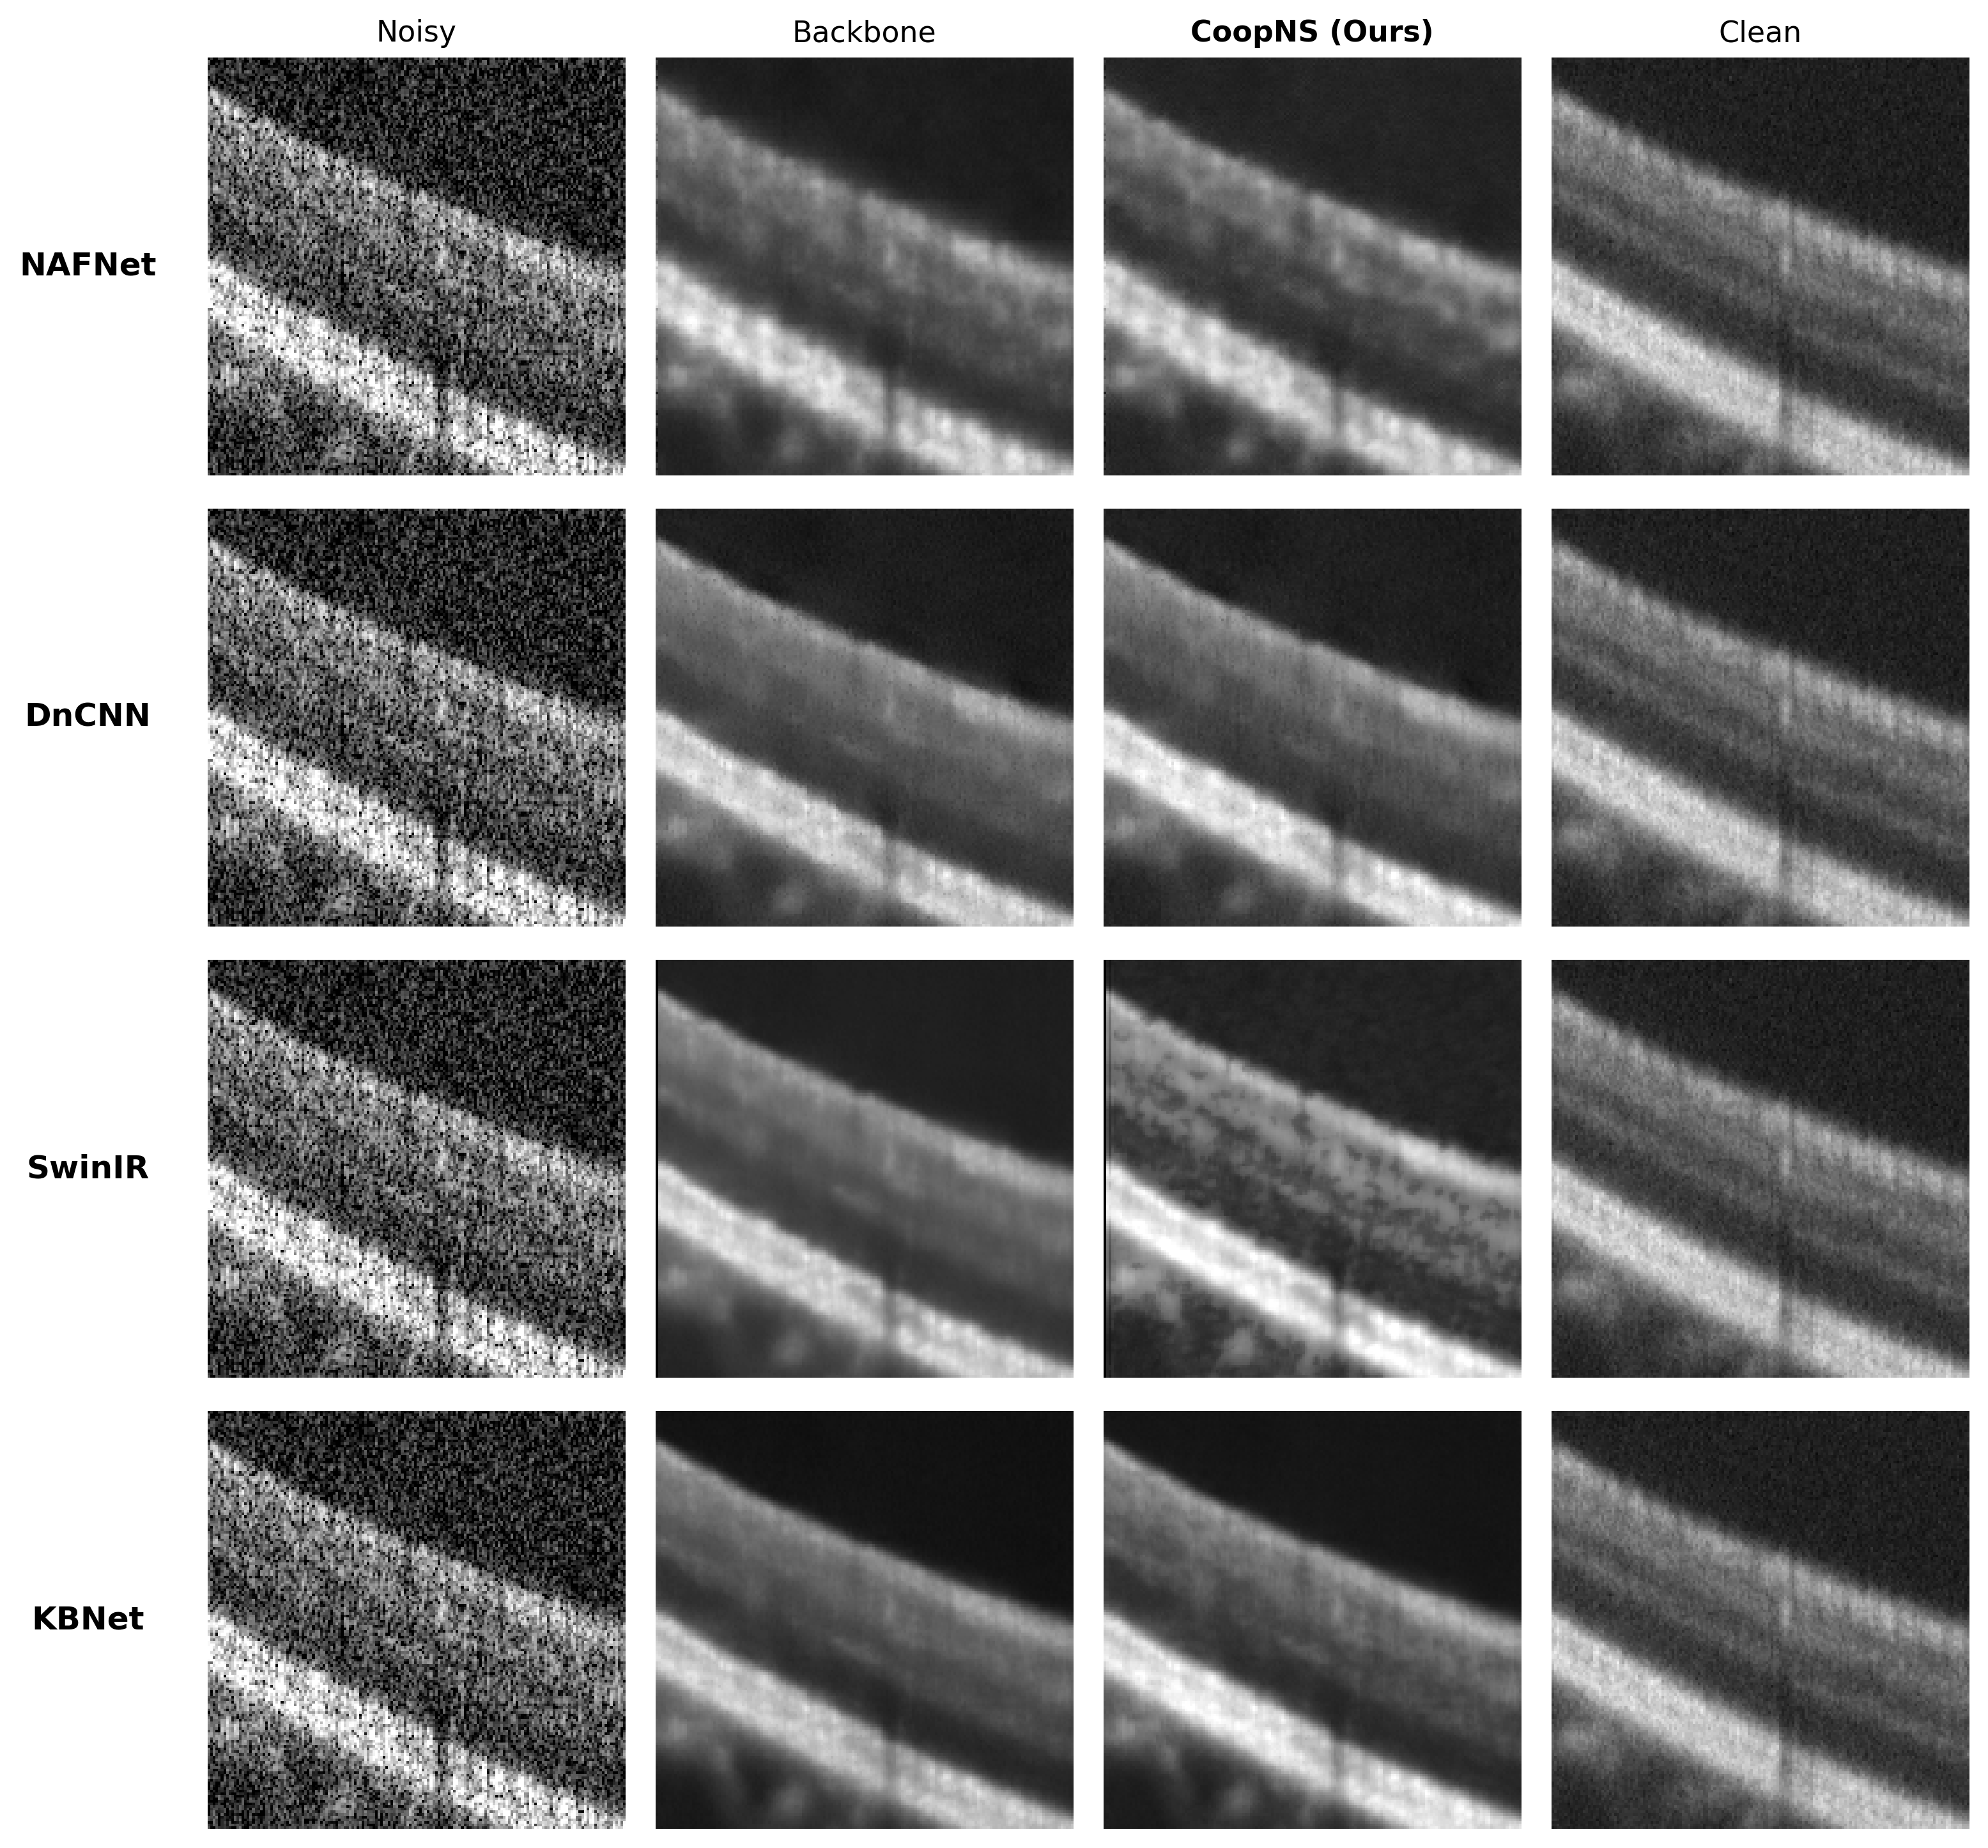
\includegraphics[width=0.52\textwidth]{figures/fig_subjective_pku37.png}
\caption{Subjective quality on PKU37 test set (in-distribution). Rows: NAFNet, DnCNN, SwinIR, KBNet. Columns: noisy input, backbone output, CoopNS-OCT-corrected output, clean reference. ROI crops use tight intensity windowing (display range [0.15, 0.85]) to visualize subtle boundary differences; this presentation choice amplifies both improvements and artifacts. Full-resolution, unwindowed images are provided in the supplementary material accompanying this submission.}
\label{fig:subjective_pku37}
\end{figure*}

\begin{figure*}[t]
\centering
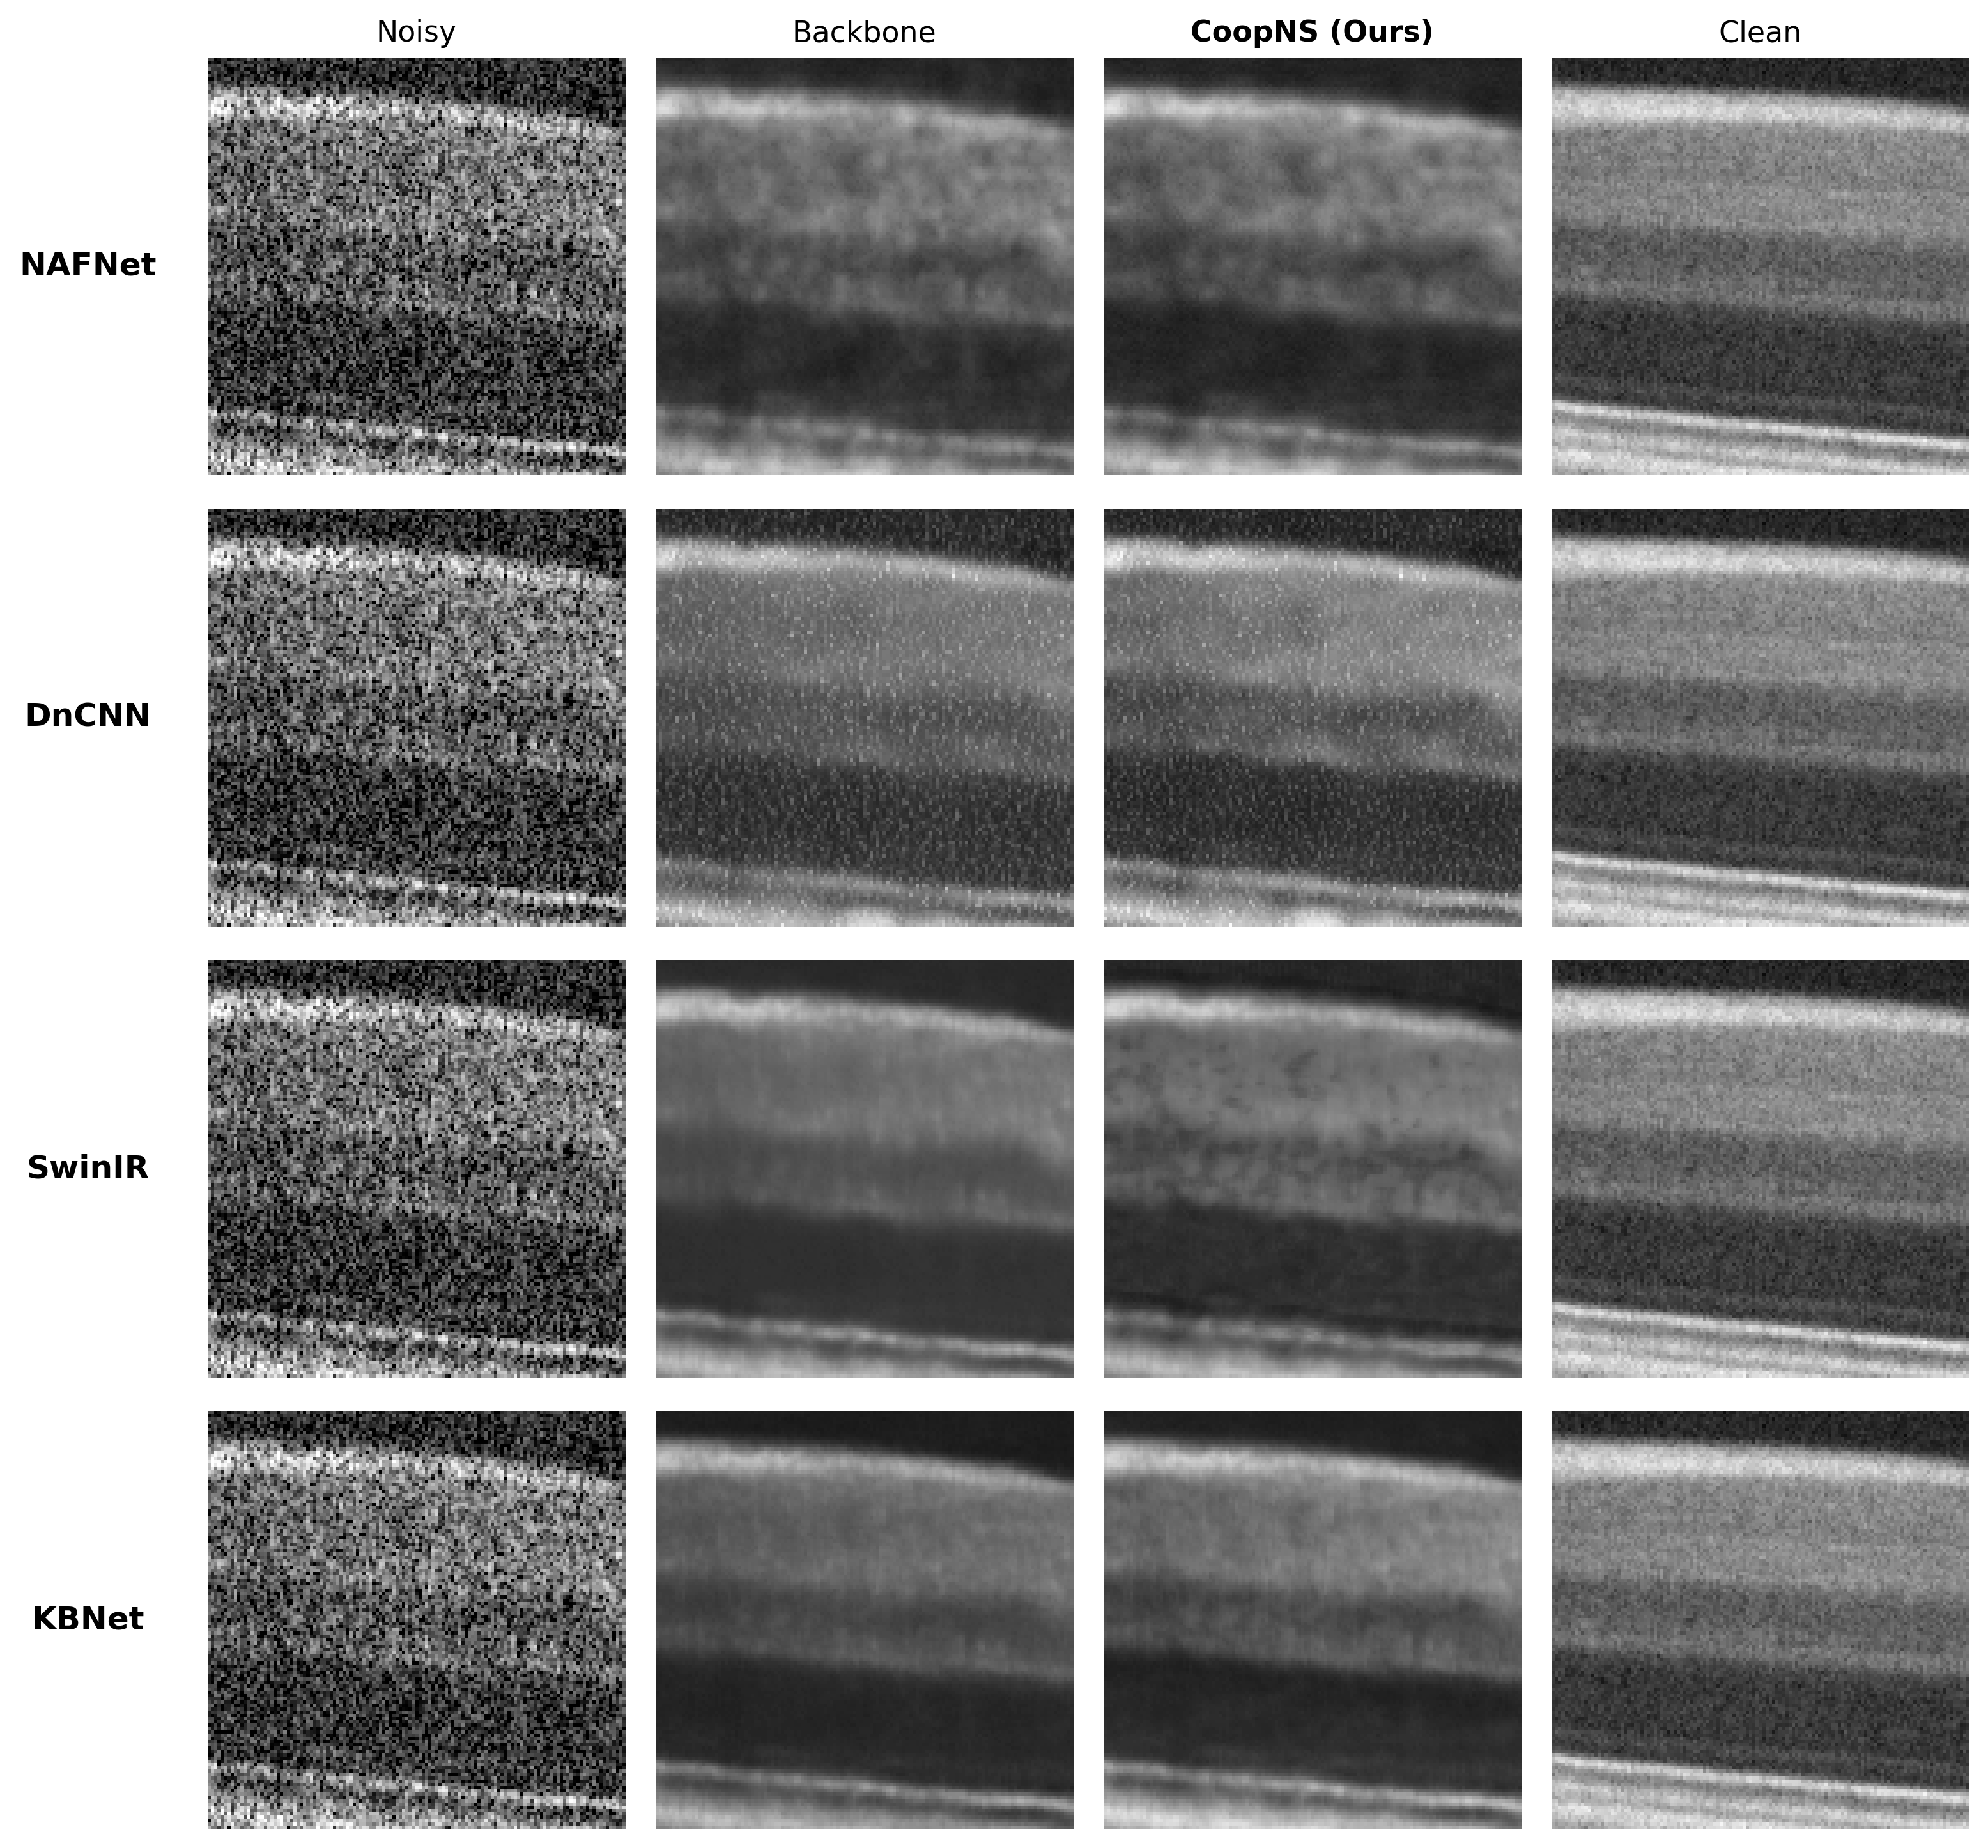
\includegraphics[width=0.52\textwidth]{figures/fig_subjective_duke17.png}
\caption{Subjective quality on Duke17 subject~9 (cross-dataset, LOO). Same layout as Fig.~\ref{fig:subjective_pku37}. CoopNS-OCT improves tissue--background contrast on out-of-distribution data from a different scanner, demonstrating cross-domain generalization.}
\label{fig:subjective_duke17}
\end{figure*}

\subsection{Cross-Dataset Generalization (LOO)}
\label{sec:results_ood}

We evaluate cross-scanner generalization via LOO cross-validation on Duke17~\cite{fang2012sparsity} (16 folds) and Duke2013~\cite{fang2013fast} (18 folds), training on $n{-}1$ images and testing on the held-out image with all four backbone families using the \emph{same} corrector architecture.

Table~\ref{tab:duke17_loo} reports LOO results on both cross-dataset benchmarks. Several observations merit discussion.

\textbf{Consistent CNR improvement.} All backbones achieve CNR gains of $+10$--$15\%$ on both benchmarks with controlled PSNR trade-off (-0.25 to -0.80\,dB), confirming cross-scanner generalization even though the corrector was trained exclusively on PKU37 data. The standard deviations across LOO folds are small relative to the mean improvements (e.g., CNR $\pm$ 2--4\% vs.\ means of $+10$--$15\%$), indicating stable corrections across subjects rather than memorized scanner-specific patterns.

\textbf{Complementary backbone profiles.} The corrector amplifies each backbone's distinct strengths. SwinIR+CoopNS-OCT achieves the highest TCI gains ($+38.9\%$ Duke17, $+25.5\%$ Duke2013), recovering tissue contrast suppressed by window-based self-attention during MSE training. DnCNN+CoopNS-OCT excels in noise suppression (ENL $+38.8\%$/$+37.8\%$) and edge recovery (EPI $+14.0\%$) but shows decreased TCI (-11.8\%/-11.1\%). Crucially, this apparent degradation is \emph{clinically beneficial}. TCI${}=1.0$ is the ideal value (perfect gradient preservation relative to the clean reference). NAFNet, SwinIR, and KBNet produce TCI$\,{<}\,1.0$ on cross-dataset data (gradients under-preserved due to over-smoothing), so the corrector increases TCI toward~1.0 (positive~$\Delta$). DnCNN, however, is the weakest cross-dataset denoiser (PSNR~24\,dB vs.\ 27\,dB for NAFNet) and leaves substantial residual speckle whose high-frequency content inflates Sobel-Y magnitude, yielding TCI$\,{>}\,1.0$ ($\text{TCI}_\text{backbone} = 1.32$ on Duke17). The corrector correctly suppresses this residual noise, reducing TCI from~1.32 toward~1.17---moving \emph{closer} to the ideal. The distance from TCI${}=1.0$ decreases for DnCNN ($0.32 \to 0.17$) just as it does for all other backbones. On in-distribution PKU37 where DnCNN TCI$_\text{backbone} = 0.64 < 1.0$, the corrector correctly increases TCI ($+4.5\%$). All other DnCNN cross-dataset metrics remain positive or strongly positive. KBNet+CoopNS-OCT dominates boundary sharpness (BS $+6.7\%$/$+10.5\%$), reflecting complementarity between kernel basis features and multiplicative gain.

\textbf{ID-to-OOD consistency.} CNR improvement narrows only slightly from the in-distribution range ($+9.7$--$15.1\%$) to the out-of-distribution range ($+10.2$--$15.1\%$), while PSNR trade-offs remain comparable. This indicates that the negotiated policy is not tied to a single scanner domain.

\textbf{Per-backbone clinical profiles.} NAFNet, KBNet, and SwinIR achieve positive $\Delta$TCI on both benchmarks (TCI$_\text{backbone} < 1.0$, corrected toward ideal). DnCNN shows negative $\Delta$TCI (-11.8\%/-11.1\%), but this reflects beneficial noise suppression: TCI$_\text{backbone} > 1.0$ due to residual speckle, and the corrector moves it toward the ideal (distance from TCI${}=1.0$: $0.32 \to 0.17$). All four backbones thus improve TCI in the \emph{same direction} (toward~1.0); the sign difference is an artifact of the $\Delta\%$ metric. We report raw $\Delta\%$ transparently and emphasize per-backbone results (Table~\ref{tab:duke17_loo}) as the primary evidence, since practitioners deploy a single backbone; the cross-backbone average is positive for all metrics on both benchmarks.

\textbf{Generalization interpretation.} The corrector has only 0.168M trainable parameters and the symbolic rules depend on local contrast, edge, smoothness, speckle, and anatomical cues rather than scanner-specific metadata. The LOO results therefore support the claim that the wrapper captures transferable quality patterns rather than memorizing a single device domain.

\begin{table*}[t]
\centering
\caption{Cross-dataset generalization via leave-one-out cross-validation. Top: Duke17 (16 subjects); Bottom: Duke2013 (18 subjects). $\Delta$PSNR in dB; other metrics in $\Delta\%$.}
\label{tab:duke17_loo}
\resizebox{\textwidth}{!}{%
\begin{tabular}{lccccccc}
\toprule
& PSNR $\Delta$ (dB) & CNR $\Delta\%$ & TCI $\Delta\%$ & EPI $\Delta\%$ & BS $\Delta\%$ & ENL $\Delta\%$ & SNR $\Delta\%$ \\
\midrule
\multicolumn{8}{l}{\textit{Duke17 (16-fold LOO)}} \\
NAFNet + CoopNS-OCT & -0.40${\pm}$0.39 & $\mathbf{+10.27{\pm}2.13}$ & $\mathbf{+7.38{\pm}4.33}$ & $\mathbf{+1.88{\pm}0.75}$ & $\mathbf{+3.15{\pm}3.97}$ & +5.46${\pm}$16.27 & -3.16${\pm}$7.89 \\
KBNet + CoopNS-OCT & -0.39${\pm}$0.70 & $\mathbf{+12.05{\pm}1.92}$ & $\mathbf{+13.43{\pm}3.31}$ & -0.66${\pm}$0.60 & $\mathbf{+6.71{\pm}4.44}$ & $\mathbf{+12.72{\pm}10.99}$ & $\mathbf{+6.31{\pm}6.69}$ \\
DnCNN + CoopNS-OCT & -0.25${\pm}$0.41 & $\mathbf{+11.62{\pm}3.49}$ & -11.76${\pm}$4.45 & $\mathbf{+14.00{\pm}8.12}$ & +3.06${\pm}$7.36 & $\mathbf{+38.75{\pm}6.27}$ & $\mathbf{+18.28{\pm}4.06}$ \\
SwinIR + CoopNS-OCT & -0.71${\pm}$0.63 & $\mathbf{+10.20{\pm}3.65}$ & $\mathbf{+38.94{\pm}10.81}$ & $\mathbf{+3.61{\pm}3.61}$ & $\mathbf{+7.42{\pm}4.30}$ & $\mathbf{+11.95{\pm}14.50}$ & -3.12${\pm}$7.54 \\
\textit{Cross-backbone mean} & -0.44 & +11.02 & +12.00 & +4.71 & +5.09 & +17.22 & +4.58 \\
\midrule
\multicolumn{8}{l}{\textit{Duke2013 (18-fold LOO)}} \\
NAFNet + CoopNS-OCT & -0.47${\pm}$0.32 & $\mathbf{+12.86{\pm}2.58}$ & $\mathbf{+9.11{\pm}3.27}$ & $\mathbf{+1.44{\pm}1.43}$ & $\mathbf{+3.76{\pm}2.91}$ & +1.32${\pm}$15.19 & -5.59${\pm}$8.24 \\
KBNet + CoopNS-OCT & -0.42${\pm}$0.59 & $\mathbf{+13.47{\pm}2.13}$ & $\mathbf{+12.45{\pm}2.16}$ & -1.04${\pm}$0.34 & $\mathbf{+10.52{\pm}3.56}$ & $\mathbf{+12.90{\pm}7.29}$ & $\mathbf{+6.72{\pm}4.42}$ \\
DnCNN + CoopNS-OCT & -0.52${\pm}$0.38 & $\mathbf{+15.05{\pm}2.34}$ & -11.12${\pm}$6.59 & $\mathbf{+4.16{\pm}2.09}$ & $\mathbf{+2.55{\pm}3.80}$ & $\mathbf{+37.81{\pm}10.53}$ & $\mathbf{+14.74{\pm}5.47}$ \\
SwinIR + CoopNS-OCT & -0.80${\pm}$0.92 & $\mathbf{+11.79{\pm}2.99}$ & $\mathbf{+25.47{\pm}11.86}$ & $\mathbf{+3.55{\pm}1.95}$ & $\mathbf{+4.26{\pm}3.40}$ & $\mathbf{+18.03{\pm}12.04}$ & +0.61${\pm}$6.23 \\
\textit{Cross-backbone mean} & -0.55 & +13.29 & +8.98 & +2.03 & +5.27 & +17.52 & +4.12 \\
\bottomrule
\end{tabular}}
\end{table*}

\subsection{Ablation Study}
\label{sec:ablation}

We ablate the key components of CoopNS-OCT using the NAFNet backbone on the PKU37 test set (173~images). Table~\ref{tab:ablation} reports delta metrics relative to the backbone-only output.

\begin{table}[t]
\centering
\caption{Ablation study on PKU37 (NAFNet backbone). $\Delta$PSNR in dB; others in $\Delta\%$.}
\label{tab:ablation}
\setlength{\tabcolsep}{2.5pt}
\footnotesize
\begin{tabular}{lcccccc}
\toprule
Config. & $\Delta$PSNR & $\Delta$CNR & $\Delta$TCI & $\Delta$EPI & $\Delta$BS & $\Delta$ENL \\
\midrule
Full & -1.09 & +12.5 & +11.4 & +0.3 & +4.1 & +29.4 \\
w/o Negotiator & -1.01 & +10.8 & +13.5 & +0.3 & +4.1 & +4.6 \\
w/o Edge Rec. & -0.62 & +7.5 & +7.0 & +0.7 & +6.8 & +2.6 \\
w/o Uncert. & -0.94 & +13.5 & +8.6 & +0.7 & +3.2 & +27.4 \\
\bottomrule
\end{tabular}
\end{table}

\textbf{Edge recovery} is the most impactful component: removing it causes the largest drops in CNR ($+12.5 \to +7.5\%$) and ENL ($+29.4 \to +2.6\%$). Without additive edge corrections, the gain corrector attempts boundary restoration through multiplicative adjustments, which boosts EPI/BS but at the cost of substantially reduced speckle suppression. This confirms that separating boundary recovery (additive) from contrast enhancement (multiplicative) is architecturally important.

\textbf{The symbolic negotiator} primarily coordinates speckle suppression---without it, ENL drops from $+29.4\%$ to $+4.6\%$. TCI \emph{increases} slightly without the negotiator ($+13.5\%$ vs.\ $+11.4\%$) because unrestricted gain boosts contrast everywhere; the negotiator trades a small amount of raw contrast for substantially better speckle suppression.

\textbf{Uncertainty guidance} focuses corrections on structurally important regions; without it, corrections spread uniformly, yielding higher CNR ($+13.5\%$) but lower TCI ($+8.6\%$ vs.\ $+11.4\%$) and BS ($+3.2\%$ vs.\ $+4.1\%$). The higher CNR without uncertainty is misleading: uniform corrections inflate the CNR numerator at the cost of reduced tissue contrast and boundary sharpness.

No single ablation variant dominates across all metrics, confirming each component addresses a distinct aspect of the quality--fidelity balance.

%% =====================================================================
%% VII. DISCUSSION
%% =====================================================================
\section{Discussion}
\label{sec:discussion}

\textbf{Why this is more than a component combination.}
The paper does not argue that edge filters, confidence maps, or fuzzy operators are individually new. The claim is that a clinically constrained OCT correction layer can be made \emph{explicit, stable, and transferable}: explicit through Table~\ref{tab:predicates}, stable through Theorem~\ref{thm:allocation_stability} and Corollary~\ref{cor:cnr}, and transferable through the four-backbone evaluation. That combination---formal predicate maps, symbolic routing, and safety-gated correction attached to pretrained backbones---is the actual technical object being studied.

\textbf{Interpretability.}
For each corrected pixel, the wrapper exposes the confidence term, the active failure maps, the compound rule activations, and the final allocation. This is materially different from a learned residual branch whose routing is implicit in feature activations alone.

\textbf{Limitations.}
The bounded correction range means that the wrapper cannot fully repair severe backbone failures. The DnCNN results also show that some metrics require careful interpretation: negative $\Delta$TCI on the OOD sets reflects a movement toward the ideal value 1.0 rather than a clinically harmful failure. Finally, the present submission is limited to the datasets and experiments already available in the repository; it does not include new reader studies or new simulations.
%% =====================================================================
%% VIII. CONCLUSION
%% =====================================================================
\section{Conclusion}
\label{sec:conclusion}

We presented CoopNS-OCT as a clinically constrained post-correction layer for OCT denoising rather than as a new denoising backbone. The paper's contribution is threefold: explicit mathematical definitions for the negotiator inputs, a stable neuro-symbolic allocation rule with a formal perturbation bound, and a safety-gated correction mechanism with a margin-based CNR guarantee. Across PKU37, Duke17 LOO, and Duke2013 LOO, the wrapper consistently improves clinically relevant metrics with modest parameter overhead and controlled PSNR cost.

The evidence supports a backbone-\emph{modular} conclusion: the same cooperative logic improves NAFNet, DnCNN, SwinIR, and KBNet after only adapting the confidence head. Future work should test whether the same formulation extends to volumetric OCT and whether the predicate family can be refined with clinician-in-the-loop validation, but the present submission already establishes that clinically meaningful post-correction can be formalized and evaluated as a rigorous technical object rather than a loose combination of existing components.


%% =====================================================================
%% REFERENCES
%% =====================================================================
{\small
\begin{thebibliography}{32}

\bibitem{huang1991optical}
D.~Huang, E.~A.~Swanson, C.~P.~Lin, J.~S.~Schuman, W.~G.~Stinson, W.~Chang, M.~R.~Hee, T.~Flotte, K.~Gregory, C.~A.~Puliafito, and J.~G.~Fujimoto, ``Optical coherence tomography,'' \emph{Science}, vol.~254, no.~5035, pp.~1178--1181, 1991.

\bibitem{goodman2007speckle}
J.~W.~Goodman, \emph{Speckle Phenomena in Optics: Theory and Applications}.\hskip 1em plus 0.5em minus 0.4em Roberts \& Company, 2007.

\bibitem{devalla2018drunet}
S.~K.~Devalla, P.~K.~Renukanand, B.~K.~Sreedhar, G.~Subramanian, L.~Zhang, S.~Perera, J.-M.~Mari, K.~S.~Chin, T.~A.~Tun, N.~G.~Strouthidis, and M.~J.~A.~Girard, ``DRUNET: A dilated-residual U-Net deep learning network to segment optic nerve head tissues in optical coherence tomography images,'' \emph{Biomed.\ Opt.\ Express}, vol.~9, no.~7, pp.~3244--3265, 2018.

\bibitem{zhang2017beyond}
K.~Zhang, W.~Zuo, Y.~Chen, D.~Meng, and L.~Zhang, ``Beyond a Gaussian denoiser: Residual learning of deep CNN for image denoising,'' \emph{IEEE Trans.\ Image Process.}, vol.~26, no.~7, pp.~3142--3155, 2017.

\bibitem{chen2022simple}
L.~Chen, X.~Chu, X.~Zhang, and J.~Sun, ``Simple baselines for image restoration,'' in \emph{Proc.\ ECCV}, 2022, pp.~17--33.

\bibitem{liang2021swinir}
J.~Liang, J.~Cao, G.~Sun, K.~Zhang, L.~Van~Gool, and R.~Timofte, ``SwinIR: Image restoration using Swin Transformer,'' in \emph{Proc.\ ICCV Workshops}, 2021, pp.~1833--1844.

\bibitem{krull2019noise2void}
A.~Krull, T.-O.~Buchholz, and F.~Jug, ``Noise2Void---learning denoising from single noisy images,'' in \emph{Proc.\ CVPR}, 2019, pp.~2129--2137.

\bibitem{rodriguez2020generalized}
A.~Rodriguez-Molares, O.~M.~H.~Rindal, J.~D'hooge, S.-E.~Masoy, A.~Austeng, M.~A.~Lediju~Bell, and H.~Torp, ``The generalized contrast-to-noise ratio: A formal definition for lesion detectability,'' \emph{IEEE Trans.\ Ultrason., Ferroelectr., Freq.\ Control}, vol.~67, no.~4, pp.~745--759, 2020.

\bibitem{defauw2018clinical}
J.~De~Fauw, J.~R.~Ledsam, B.~Romera-Paredes, \emph{et~al.}, ``Clinically applicable deep learning for diagnosis and referral in retinal disease,'' \emph{Nature Med.}, vol.~24, pp.~1342--1350, 2018.

\bibitem{vankrieken2022analyzing}
E.~van~Krieken, E.~Acar, and F.~van~Harmelen, ``Analyzing differentiable fuzzy logic operators,'' \emph{Artif.\ Intell.}, vol.~302, art.~103602, 2022.

\bibitem{zhang2023kbnet}
Y.~Zhang, D.~Li, X.~Shi, D.~He, K.~Song, X.~Wang, H.~Qin, and H.~Li, ``KBNet: Kernel basis network for image restoration,'' Tech.\ Rep.\ arXiv:2303.02881, 2023. [Online]. Available: \url{https://arxiv.org/abs/2303.02881}

\bibitem{buades2005non}
A.~Buades, B.~Coll, and J.-M.~Morel, ``A non-local algorithm for image denoising,'' in \emph{Proc.\ CVPR}, vol.~2, 2005, pp.~60--65.

\bibitem{mayer2012wavelet}
M.~A.~Mayer, A.~Borsdorf, M.~Wagner, J.~Hornegger, C.~Y.~Mardin, and R.~P.~Tornow, ``Wavelet denoising of multiframe optical coherence tomography data,'' \emph{Biomed.\ Opt.\ Express}, vol.~3, no.~3, pp.~572--589, 2012.

\bibitem{geng2022triplet}
M.~Geng, X.~Meng, L.~Zhu, Z.~Jiang, M.~Gao, Z.~Huang, B.~Qiu, Y.~Hu, Y.~Zhang, Q.~Ren, and Y.~Lu, ``Triplet cross-fusion learning for unpaired image denoising in optical coherence tomography,'' \emph{IEEE Trans.\ Med.\ Imag.}, vol.~41, no.~11, pp.~3357--3372, 2022.

\bibitem{fang2012sparsity}
L.~Fang, S.~Li, Q.~Nie, J.~A.~Izatt, C.~A.~Toth, and S.~Farsiu, ``Sparsity based denoising of spectral domain optical coherence tomography images,'' \emph{Biomed.\ Opt.\ Express}, vol.~3, no.~5, pp.~927--942, 2012.

\bibitem{fang2013fast}
L.~Fang, S.~Li, R.~P.~McNabb, Q.~Nie, A.~N.~Kuo, C.~A.~Toth, J.A.~Izatt, and S.~Farsiu, ``Fast acquisition and reconstruction of optical coherence tomography images via sparse representation,'' \emph{IEEE Trans.\ Med.\ Imag.}, vol.~32, no.~11, pp.~2034--2049, 2013.

\bibitem{wang2019quality}
J.~Wang, G.~Deng, W.~Li, Y.~Chen, F.~Gao, H.~Liu, Y.~He, and G.~Shi, ``Deep learning for quality assessment of retinal OCT images,'' \emph{Biomed.\ Opt.\ Express}, vol.~10, no.~12, pp.~6057--6072, 2019.

\bibitem{gal2016dropout}
Y.~Gal and Z.~Ghahramani, ``Dropout as a Bayesian approximation: Representing model uncertainty in deep learning,'' in \emph{Proc.\ ICML}, 2016, pp.~1050--1059.

\bibitem{kendall2018multi}
A.~Kendall, Y.~Gal, and R.~Cipolla, ``Multi-task learning using uncertainty to weigh losses for scene geometry and semantics,'' in \emph{Proc.\ CVPR}, 2018, pp.~7482--7491.

\bibitem{lakshminarayanan2017simple}
B.~Lakshminarayanan, A.~Pritzel, and C.~Blundell, ``Simple and scalable predictive uncertainty estimation using deep ensembles,'' in \emph{Proc.\ NeurIPS}, 2017, pp.~6402--6413.

\bibitem{garcez2023neurosymbolic}
A.~d'Avila~Garcez and L.~C.~Lamb, ``Neurosymbolic AI: The 3rd wave,'' \emph{Artif.\ Intell.\ Rev.}, vol.~56, pp.~12387--12406, 2023.

\bibitem{fdaaiml2021}
U.S.\ Food and Drug Administration, ``Artificial intelligence/machine learning (AI/ML)-based software as a medical device (SaMD) action plan,'' FDA, Jan.\ 2021.

\bibitem{stein2006quality}
D.~M.~Stein, H.~Ishikawa, R.~Hariprasad, G.~Wollstein, R.~J.~Noecker, J.~G.~Fujimoto, and J.~S.~Schuman, ``A new quality assessment parameter for optical coherence tomography,'' \emph{Br.\ J.\ Ophthalmol.}, vol.~90, no.~2, pp.~186--190, 2006.

\bibitem{tewarie2012oscar}
P.~Tewarie, L.~Balk, F.~Costello, A.~Green, R.~Martin, S.~Schippling, and A.~Petzold, ``The OSCAR-IB consensus criteria for retinal OCT quality assessment,'' \emph{PLoS ONE}, vol.~7, no.~4, art.~e34823, 2012.

\bibitem{kingma2015adam}
D.~P.~Kingma and J.~Ba, ``Adam: A method for stochastic optimization,'' in \emph{Proc.\ ICLR}, 2015.

\bibitem{wang2004image}
Z.~Wang, A.~C.~Bovik, H.~R.~Sheikh, and E.~P.~Simoncelli, ``Image quality assessment: From error visibility to structural similarity,'' \emph{IEEE Trans.\ Image Process.}, vol.~13, no.~4, pp.~600--612, 2004.

\bibitem{loshchilov2019decoupled}
I.~Loshchilov and F.~Hutter, ``Decoupled weight decay regularization,'' in \emph{Proc.\ ICLR}, 2019.

\bibitem{gonzalez2018digital}
R.~C.~Gonzalez and R.~E.~Woods, \emph{Digital Image Processing}, 4th~ed.\hskip 1em plus 0.5em minus 0.4em Pearson, 2018.

\bibitem{zuiderveld1994clahe}
K.~Zuiderveld, ``Contrast limited adaptive histogram equalization,'' in \emph{Graphics Gems IV}, P.~S.~Heckbert, Ed.\hskip 1em plus 0.5em minus 0.4em Academic Press, 1994, pp.~474--485.

\bibitem{tomasi1998bilateral}
C.~Tomasi and R.~Manduchi, ``Bilateral filtering for gray and color images,'' in \emph{Proc.\ ICCV}, 1998, pp.~839--846.

\bibitem{polesel2000image}
A.~Polesel, G.~Ramponi, and V.~J.~Mathews, ``Image enhancement via adaptive unsharp masking,'' \emph{IEEE Trans.\ Image Process.}, vol.~9, no.~3, pp.~505--510, 2000.

\bibitem{cohen1988statistical}
J.~Cohen, \emph{Statistical Power Analysis for the Behavioral Sciences}, 2nd~ed.\hskip 1em plus 0.5em minus 0.4em Lawrence Erlbaum Associates, 1988.

\end{thebibliography}
}

\end{document}
